\chapter{Lists}

\textsc{Perspective}:Most programming languages support some form of
vector or array data type in which elements can be referenced by
position. Icon's list data type fills this need, but it differs from
similar types in many languages in that Icon lists are constructed
during program execution instead of being declared during
compilation. Therefore, the size of a list may not be known until run
time.

Icon's lists are data objects. They can be assigned to variables and
passed as arguments to functions. They are not copied when this is
done; in fact, a value of type list is simply a descriptor that points
to the structure that contains the list elements. These aspects of
lists are shared by several other Icon data types and do not add
anything new to the implementation. The attribute of lists that
presents the most challenging implementation problem is their ability
to grow and shrink by the use of stack and queue access mechanisms.

Lists present different faces to the programmer, depending on how they
are used. They may be static vectors referenced by position or they
may be dynamic changing stacks or queues. It might seem that having a
data structure with such apparently discordant access mechanisms would
be awkward and undesirable. In practice, Icon's lists provide a
remarkably flexible mechanism for dealing with many common programming
problems. The two ways of manipulating lists are rarely
intermixed. When both aspects are needed, they usually are needed at
different times. For example, the number of elements needed in a list
often is not known when the list is created. Such a list can be
created with no elements, and the elements can be pushed onto it as
they are produced. Once such a list has been constructed, it may be
accessed by position with no further change in its size.

\section[6.1 Structures for Lists]{6.1 Structures for Lists}

The fusion of vector, stack, and queue organizations is reflected in
the implementation of Icon by relatively complicated structures that
are designed to provide a reasonable compromise between the
conflicting requirements of the different access mechanisms.


A list consists of a fixed-size \textit{list-header block}, which
contains the usual title, the current size of the list (the number of
elements in it), and block pointers that point to the first and last
blocks on a doubly-linked chain of \textit{list-element blocks} that
contain the actual list elements. List-element blocks vary in size.


A list-element block contains the usual title, the size of the block
in bytes three words used to determine the locations of elements in
the list-element block and block pointers that point to the next and
previous list-element blocks, if any. A null pointer
\textcolor[rgb]{0.0,0.2784314,1.0}{(in Unicon, a pointer back to the
list header block)} indicates the absence of a pointer to another
list-element block. Following this data, there are slots for
elements. Slots always contain valid descriptors, even if they are not
used to hold list elements.


The structure declarations for list-header blocks and list-element blocks are

%-% {\ttfamily\mdseries
%-% \ \ \ struct b\_list \{\ \ /* list-header block */}
%-% 
%-% {\ttfamily\mdseries
%-% \ \ \ \ \ \ word title;\ \ /*\ \ T\_List */}
%-% 
%-% {\ttfamily\mdseries
%-% \ \ \ \ \ \ word size;\ \ /*\ \ current list size */}
%-% 
%-% {\ttfamily\mdseries
%-% \ \ \ \ \ \ word id;\ \ \ \ /*\ \ identification number */}
%-% 
%-% {\ttfamily\mdseries
%-% \ \ \ \ \ \ union block *listhead; /* first list-element block \textit{*}/}
%-% 
%-% {\ttfamily\mdseries
%-% \ \ \ \ \ \ union block *listtail; /* last list-element block \textit{*}/}
%-% 
%-% {\ttfamily\mdseries
%-% \ \ \ \};}
%-% 
%-% {\ttfamily\mdseries
%-% \ \ \ struct b\_lelem \{\ \ /* list-element block */}
%-% 
%-% {\ttfamily\mdseries
%-% \ \ \ \ \ \ word title;\ \ /*\ \ T\_Lelem */}
%-% 
%-% {\ttfamily\mdseries
%-% \ \ \ \ \ \ word blksize;\ \ /*\ \ size of block */}
%-% 
%-% {\ttfamily\mdseries
%-% \ \ \ \ \ \ word nslots;\ \ /*\ \ total number of slots */}
%-% 
%-% {\ttfamily\mdseries
%-% \ \ \ \ \ \ word first;\ \ /*\ \ index of first used slot */}
%-% 
%-% {\ttfamily\mdseries
%-% \ \ \ \ \ \ word nused;\ \ /*\ \ number of used slots */}
%-% 
%-% {\ttfamily\mdseries
%-% \ \ \ \ \ \ union block *listprev; \ /* previous list-element block */}
%-% 
%-% {\ttfamily\mdseries
%-% \ \ \ \ \ \ union block *listnext; \ /* next list-element block */}
%-% 
%-% {\ttfamily\mdseries
%-% \ \ \ \ \ \ struct descrip lslots[1]; /* array of slots */}
%-% 
%-% {\ttfamily\mdseries
%-% \ \ \ \};}
\iconcode{
\>struct b\_list \{\>\>\>\>\>\>\>/* list-header block */\\
\>\>word title;\>\>\>\>\>\>\>/*\ \ T\_List */\\
\>\>word size;\>\>\>\>\>\>\>/*\ \ current list size */\\
\>\>word id;\>\>\>\>\>\>\>/*\ \ identification number */\\
\>\>union block *listhead;\>\>\>\>\>\>\>/* first list-element block \textit{*}/\\
\>\>union block *listtail;\>\>\>\>\>\>\>/* last list-element block \textit{*}/\\
\>\};\\
\>struct b\_lelem \{\>\>\>\>\>\>\>/* list-element block */\\
\>\>word title;\>\>\>\>\>\>\>/*\ \ T\_Lelem */\\
\>\>word blksize;\>\>\>\>\>\>\>/*\ \ size of block */\\
\>\>word nslots;\>\>\>\>\>\>\>/*\ \ total number of slots */\\
\>\>word first;\>\>\>\>\>\>\>/*\ \ index of first used slot */\\
\>\>word nused;\>\>\>\>\>\>\>/*\ \ number of used slots */\\
\>\>union block *listprev;\>\>\>\>\>\>\>/* previous list-element block */\\
\>\>union block *listnext;\>\>\>\>\>\>\>/* next list-element block */\\
\>\>struct descrip lslots[1];\>\>\>\>\>\>\>/* array of slots */\\
\>\};
}

When a list is created, either by

%-% {\ttfamily\mdseries
%-% \ \ \ list(n, x)}
\iconline{
\>list(n, x)
}

\noindent or by

%-% {\ttfamily\mdseries
%-% \ \ \ [x1 ,x2, ..., xn]}
\iconline{
\>[x1 ,x2, ..., xn]
}

\noindent there is only one list-element block. Other list-element
blocks may be added to the chain as the result of pushs or puts.

List-element blocks have a minimum number of slots. This allows some
expansion room for adding elements to lists, such as the empty list, that
are small initially. The minimum number of slots is given by
\texttt{MinListSlots}, which normally is eight. In the examples that
follow, the value of \texttt{MinListSlots} is assumed to be four in order
to keep the diagrams to a manageable size.

The code for the list function is

%-% {\ttfamily\mdseries
%-% function\{1\} list(n, x)}
%-% 
%-% {\ttfamily\mdseries
%-% \ \ \ if is:set(n) then \{}
%-% 
%-% {\ttfamily\mdseries
%-% \ \ \ \ \ \ abstract \{}
%-% 
%-% {\ttfamily\mdseries
%-% \ \ \ \ \ \ \ \ \ return new list(store[type(n).set\_elem])}
%-% 
%-% {\ttfamily\mdseries
%-% \ \ \ \ \ \ \ \  \}}
%-% 
%-% {\ttfamily\mdseries
%-% \ \ \ \ \ \ body \{}
%-% 
%-% {\ttfamily\mdseries
%-% \ \ \ \ \ \ \ \ \ struct descrip d;}
%-% 
%-% {\ttfamily\mdseries
%-% \ \ \ \ \ \ \ \ \ cnv\_list(\&n, \&d); /* can't fail, we know n is a set */}
%-% 
%-% {\ttfamily\mdseries
%-% \ \ \ \ \ \ \ \ \ return d;}
%-% 
%-% {\ttfamily\mdseries
%-% \ \ \ \ \ \ \ \ \ \}}
%-% 
%-% {\ttfamily\mdseries
%-% \ \ \ \ \ \ \}}
%-% 
%-% {\ttfamily\mdseries
%-% \ \ \ else \{}
%-% 
%-% {\ttfamily\mdseries
%-% \ \ \ \ \ \ if !def:C\_integer(n, 0L) then}
%-% 
%-% {\ttfamily\mdseries
%-% \ \  runerr(101, n)}
%-% 
%-% 
%-% \bigskip
%-% 
%-% {\ttfamily\mdseries
%-% \ \ \ abstract \{}
%-% 
%-% {\ttfamily\mdseries
%-% \ \ \ \ \ \ return new list(type(x))}
%-% 
%-% {\ttfamily\mdseries
%-% \ \ \ \ \ \ \}}
%-% 
%-% 
%-% \bigskip
%-% 
%-% {\ttfamily\mdseries
%-% \ \ \ body \{}
%-% 
%-% {\ttfamily\mdseries
%-% \ \ \ \ \ \ tended struct b\_list *hp;}
%-% 
%-% {\ttfamily\mdseries
%-% \ \ \ \ \ \ register word i, size;}
%-% 
%-% {\ttfamily\mdseries
%-% \ \ \ \ \ \ word nslots;}
%-% 
%-% {\ttfamily\mdseries
%-% \ \ \ \ \ \ register struct b\_lelem *bp; /* doesnt need to be tended */}
%-% 
%-% 
%-% \bigskip
%-% 
%-% {\ttfamily\mdseries
%-% \ \ \ \ \ \ nslots = size = n;}
%-% 
%-% 
%-% \bigskip
%-% 
%-% {\ttfamily\mdseries
%-% \ \ \ \ \ \ /*}
%-% 
%-% {\ttfamily\mdseries
%-% \ \ \ \ \ \ \ * Ensure that the size is positive and that the}
%-% 
%-% {\ttfamily\mdseries
%-% \ \ \ \ \ \ \ * \ list-element block has at least MinListSlots slots.}
%-% 
%-% {\ttfamily\mdseries
%-% \ \ \ \ \ \ \ */}
%-% 
%-% {\ttfamily\mdseries
%-% \ \ \ \ \ \ if (size {\textless} 0) \{}
%-% 
%-% {\ttfamily\mdseries
%-% \ \ \ \ \ \ \ \ \ irunerr(205, n);}
%-% 
%-% {\ttfamily\mdseries
%-% \ \ \ \ \ \ \ \ \ errorfail;}
%-% 
%-% {\ttfamily\mdseries
%-% \ \ \ \ \ \ \ \ \ \}}
%-% 
%-% {\ttfamily\mdseries
%-% \ \ \ \ \ \ if (nslots == 0)}
%-% 
%-% {\ttfamily\mdseries
%-% \ \ \ \ \ \ \ \ \ nslots = MinListSlots;}
%-% 
%-% {\ttfamily\mdseries
%-% \ \ \ \ \ \ /*}
%-% 
%-% {\ttfamily\mdseries
%-% \ \ \ \ \ \ \ * Allocate the list-header block and a list-element block.}
%-% 
%-% {\ttfamily\mdseries
%-% \ \ \ \ \ \ \ * \ nslots is the number of slots in the list-element}
%-% 
%-% {\ttfamily\mdseries
%-% \ \ \ \ \ \ \ * \ block while size is the number of elements in the list.}
%-% 
%-% {\ttfamily\mdseries
%-% \ \ \ \ \ \ \ */}
%-% 
%-% {\ttfamily\mdseries
%-% \ \ \ \ \ \ Protect(hp = alclist\_raw(size, nslots), runerr(0));}
%-% 
%-% {\ttfamily\mdseries
%-% \ \ \ \ \ \ bp = (struct b\_lelem *)hp-{\textgreater}listhead;}
%-% 
%-% 
%-% \bigskip
%-% 
%-% {\ttfamily\mdseries
%-% \ \ \ \ \ \ /*}
%-% 
%-% {\ttfamily\mdseries
%-% \ \ \ \ \ \ \ * Initialize each slot.}
%-% 
%-% {\ttfamily\mdseries
%-% \ \ \ \ \ \ \ */}
%-% 
%-% {\ttfamily\mdseries
%-% \ \ \ \ \ \ for (i = 0; i {\textless} size; i++)}
%-% 
%-% {\ttfamily\mdseries
%-% \ \ \ \ \ \ \ \ \ bp-{\textgreater}lslots[i] = x;}
%-% 
%-% 
%-% \bigskip
%-% 
%-% {\ttfamily\mdseries
%-% \ \ \ \ \ \ Desc\_EVValD(hp, E\_Lcreate, D\_List);}
%-% 
%-% 
%-% \bigskip
%-% 
%-% {\ttfamily\mdseries
%-% \ \ \ \ \ \ /*}
%-% 
%-% {\ttfamily\mdseries
%-% \ \ \ \ \ \ \ * Return the new list.}
%-% 
%-% {\ttfamily\mdseries
%-% \ \ \ \ \ \ \ */}
%-% 
%-% {\ttfamily\mdseries
%-% \ \ \ \ \ \ return list(hp);}
%-% 
%-% {\ttfamily\mdseries
%-% \ \ \ \ \ \ \}}
%-% 
%-% {\ttfamily\mdseries
%-% \ \ \ \}}
%-% 
%-% {\ttfamily\mdseries
%-% end}
\goodbreak
\iconcode{
function\{1\} list(n, x)\\
\>if is:set(n) then \{\\
\>\>abstract \{\\
\>\>\>return new list(store[type(n).set\_elem])\\
\>\>\ \  \}\\
\>\>body \{\\
\>\>\>struct descrip d;\\
\>\>\>cnv\_list(\&n, \&d); /* can't fail, we know n is a set */\\
\>\>\>return d;\\
\>\>\>\}\\
\>\>\}\\
\>else \{\\
\>\>if !def:C\_integer(n, 0L) then\\
\ \  runerr(101, n)\\
\\
\>abstract \{\\
\>\>return new list(type(x))\\
\>\>\}\\
\\
\>\>tended struct b\_list *hp;\\
\>\>register word i, size;\\
\>\>word nslots;\\
\>\>register struct b\_lelem *bp; /* doesnt need to be tended */\\
\\
\>\>nslots = size = n;\\
\\
\>\>/*\\
\>\>\ * Ensure that the size is positive and that the\\
\>\>\ * \ list-element block has at least MinListSlots slots.\\
\>\>\ */\\
\>\>if (size < 0) \{\\
\>\>\>irunerr(205, n);\\
\>\>\>errorfail;\\
\>\>\>\}\\
\>\>if (nslots == 0)\\
\>\>\>nslots = MinListSlots;\\
\>\>/*\\
\>\>\ * Allocate the list-header block and a list-element block.\\
\>\>\ * \ nslots is the number of slots in the list-element\\
\>\>\ * \ block while size is the number of elements in the list.\\
\>\>\ */\\
\>\>Protect(hp = alclist\_raw(size, nslots), runerr(0));\\
\>\>bp = (struct b\_lelem *)hp->listhead;\\
\\
\>\>/*\\
\>\>\ * Initialize each slot.\\
\>\>\ */\\
\>\>for (i = 0; i < size; i++)\\
\>\>\>bp->lslots[i] = x;\\
\\
\>\>Desc\_EVValD(hp, E\_Lcreate, D\_List);\\
\\
\>\>/*\\
\>\>\ * Return the new list.\\
\>\>\ */\\
\>\>return list(hp);\\
\>\>\}\\
\>\}\\
end
}

The data structures produced for a list are illustrated by the result
of evaluating

%-% {\ttfamily\mdseries
%-% \ \ \ a := list(1, 4)}
\iconline{
\>a := list(1, 4)
}

\noindent which produces a one-element list containing the value 4:

%--%\ \  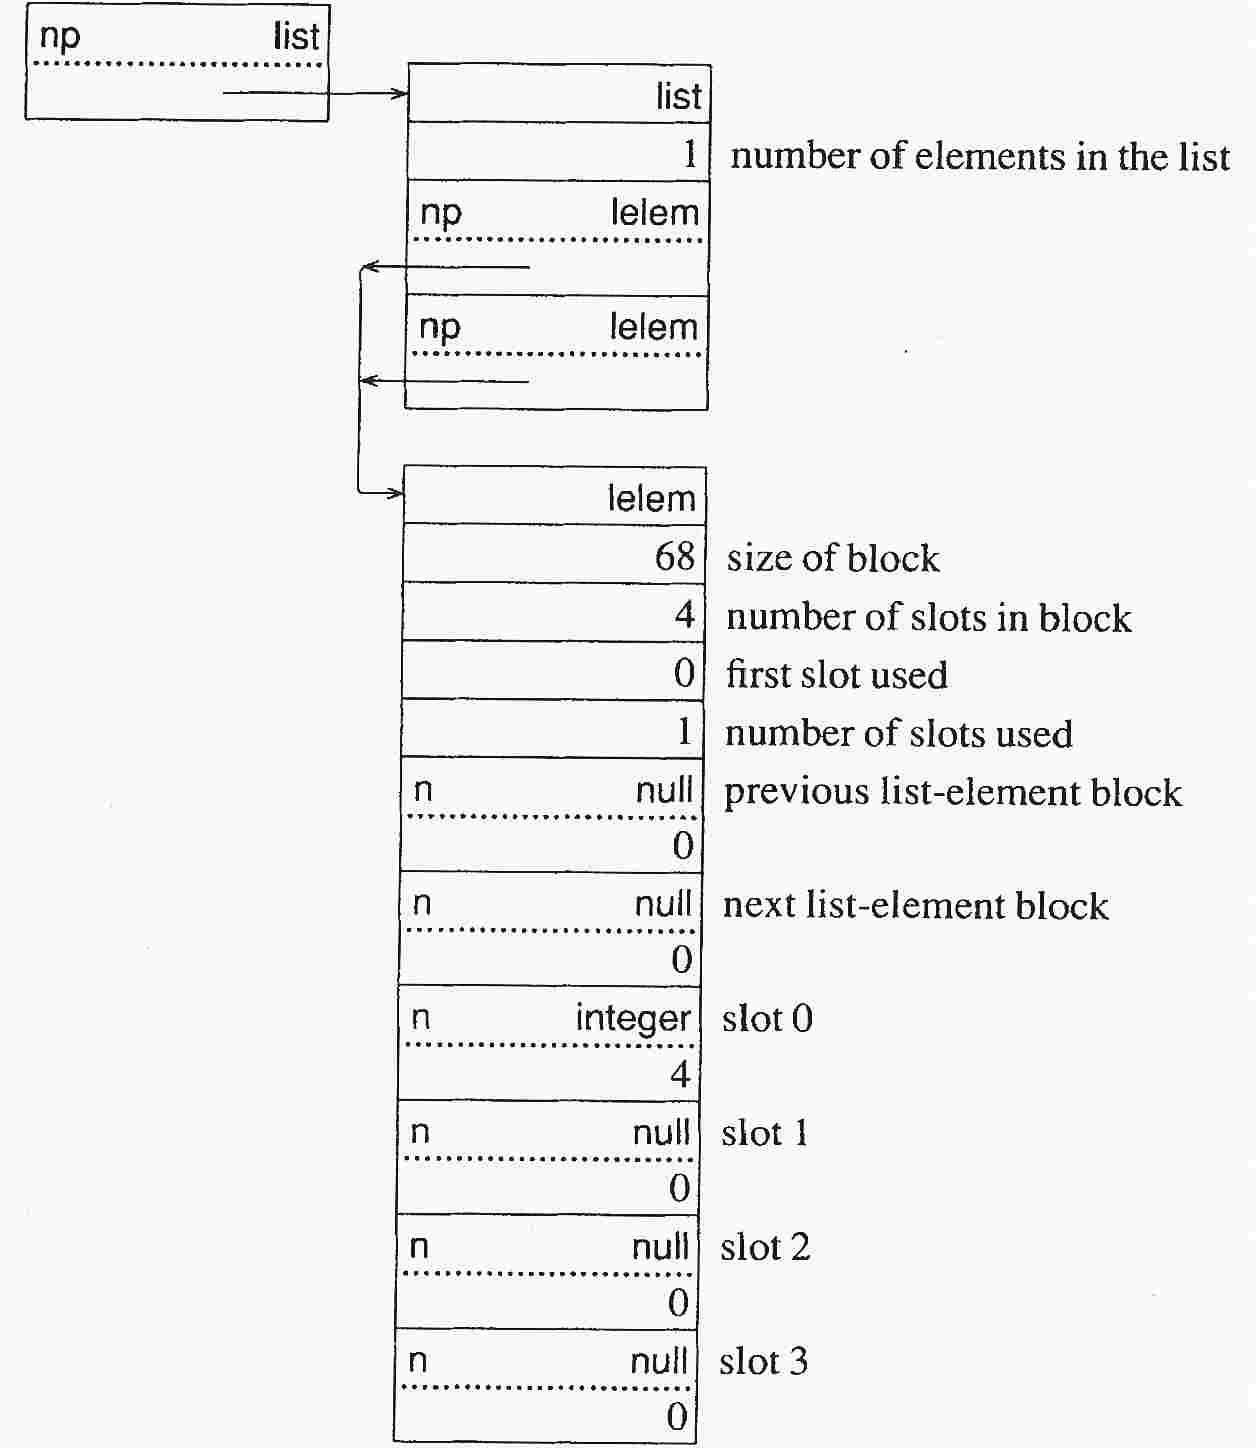
\includegraphics[width=4.2752in,height=4.8362in]{ib-img/ib-img027.jpg} 
\begin{picture}(300,360)
\put(130,0){\dvbox{null}{n}{0}}
\put(130,0){\trboxlabel{slot 3}}
\put(130,32){\dvbox{null}{n}{0}}
\put(130,32){\trboxlabel{slot 2}}
\put(130,64){\dvbox{null}{n}{0}}
\put(130,64){\trboxlabel{slot 1}}
\put(130,96){\dvbox{integer}{n}{4}}
\put(130,96){\trboxlabel{slot 0}}
\put(130,128){\nullptrbox{next list-element block}}
{\color{blue}
\put(-10,136){\parbox{100pt}{Unicon replaces the null pointer used by Icon
    with a pointer to the list header block.}}
\multiput(100,136)(4,0){30}{\line(1,0){2}}
\put(370,136){\line(1,0){50}}
\put(420,136){\line(0,1){214}}
\put(420,350){\vector(-1,0){150}}
\put(270,350){\line(-1,0){154}}
\put(116,350){\vector(0,-1){22}}
}
\put(130,144){\nullptrbox{previous list-element block}}
\begin{picture}(0,0)(0,32)
\put(130,192){\blkbox{0}{1}}
\put(130,192){\rightboxlabels{first slot used}{number of slots used}}
\put(130,224){\blkbox{60}{4}}
\put(130,224){\rightboxlabels{size of block}{number of slots in block}}
\put(130,256){\wordbox{lelem}{}}
\put(130,288){\blkbox{}{}}
\put(130,288){\rightboxlabels{first list-element block (head)}
   {last list-element block(tail)}}
\put(130,306){\lptr{40}}
\put(130,288){\lptr{40}}
\put(110,314){\line(0,-1){51}}
\put(110,263){\vector(1,0){20}}
\put(130,320){\wordbox{\textit{id}}}
\put(130,336){\blkbox{list}{1}}
\put(130,336){\brboxlabel{number of elements in the list}}
\put(0,352){\dvptrbox{list}{np}{50}{}}
\end{picture}
\end{picture}

\ \ \ \ Data Structures for \texttt{list(1,4)}

Note that there is only one list-element block and that the slot
indexing in the block is zero-based. Unused slots contain null values
that are logically inaccessible.

\section[6.2 Queue and Stack Access]{6.2 Queue and Stack Access}

Elements in a list-element block are stored as a doubly-linked
circular queue. If an element is added to the end of the list
\texttt{a}, as in

%-% {\ttfamily\mdseries
%-% \ \ \ put(a, 5)}
\iconline{
\>put(a, 5)
}

\noindent the elements of the list are 4 and 5. The value is added to
the '{\textquotedbl}end{\textquotedbl} of the last list-element block,
assuming there is an unused slot (as there is in this case). The code
in \texttt{put()} to do this is

%-% {\ttfamily\mdseries
%-% \ \ \ /*}
%-% 
%-% {\ttfamily\mdseries
%-% \ \ \ \ * Point hp to the list-header block and bp to the last}
%-% 
%-% {\ttfamily\mdseries
%-% \ \ \ \ * list-element block.}
%-% 
%-% {\ttfamily\mdseries
%-% \ \ \ \ */}
%-% 
%-% {\ttfamily\mdseries
%-% \ \ \ hp = (struct b\_list *)BlkLoc(x);}
%-% 
%-% {\ttfamily\mdseries
%-% \ \ \ bp = (struct b\_lelem *) hp-{\textgreater}listtail;}
%-% 
%-% {\ttfamily\mdseries
%-% \ \ \ /*}
%-% 
%-% {\ttfamily\mdseries
%-% \ \ \ \ * If the last list-element block is full, allocate a new}
%-% 
%-% {\ttfamily\mdseries
%-% \ \ \ \ *\ \ list-element block, make it the first list-element block,}
%-% 
%-% {\ttfamily\mdseries
%-% \ \ \ \ *\ \ and make it the next block of the former last list-element}
%-% 
%-% {\ttfamily\mdseries
%-% \ \ \ \ * block.}
%-% 
%-% {\ttfamily\mdseries
%-% \ \ \ \ */}
%-% 
%-% {\ttfamily\mdseries
%-% \ \  if (bp-{\textgreater}nused {\textgreater}= bp-{\textgreater}nslots) \{}
%-% 
%-% {\ttfamily\mdseries
%-% \ \  \ \ \ /*}
%-% 
%-% {\ttfamily\mdseries
%-% \ \  \ \ \ \ * Set i to the size of block to allocate.}
%-% 
%-% {\ttfamily\mdseries
%-% \ \  \ \ \ \ */}
%-% 
%-% {\ttfamily\mdseries
%-% \ \  \ \ \ i = hp-{\textgreater}size / two;}
%-% 
%-% {\ttfamily\mdseries
%-% \ \  \ \ \ if (i {\textless} MinListSlots)}
%-% 
%-% {\ttfamily\mdseries
%-% \ \  \ \ \ \ \ \ i = MinListSlots;}
%-% 
%-% {\ttfamily\mdseries
%-% \#ifdef MaxListSlots}
%-% 
%-% {\ttfamily\mdseries
%-% \ \  \ \ \ if (i {\textgreater} MaxListSlots)}
%-% 
%-% {\ttfamily\mdseries
%-% \ \  \ \ \ \ \ \ i = MaxListSlots;}
%-% 
%-% {\ttfamily\mdseries
%-% \#endif\ \ \ \ \ \ \ \ \ \ /* MaxListSlots */}
%-% 
%-% {\ttfamily\mdseries
%-% \ \  \ \ \ /*}
%-% 
%-% {\ttfamily\mdseries
%-% \ \  \ \ \ \ * Allocate a new list element block. \ If the block}
%-% 
%-% {\ttfamily\mdseries
%-% \ \  \ \ \ \ * \ can't be allocated, try smaller blocks.}
%-% 
%-% {\ttfamily\mdseries
%-% \ \  \ \ \ \ */}
%-% 
%-% {\ttfamily\mdseries
%-% \ \  \ \ \ while ((bp = alclstb(i, (word)0, (word)0)) == NULL) \{}
%-% 
%-% {\ttfamily\mdseries
%-% \ \  \ \ \ \ \ \ i /= 4;}
%-% 
%-% {\ttfamily\mdseries
%-% \ \  \ \ \ \ \ \ if (i {\textless} MinListSlots)}
%-% 
%-% {\ttfamily\mdseries
%-% \ \ \ \  \ runerr(0);}
%-% 
%-% {\ttfamily\mdseries
%-% \ \  \ \ \ \ \ \ \}}
%-% 
%-% 
%-% \bigskip
%-% 
%-% {\ttfamily\mdseries
%-% \ \  \ \ \ hp-{\textgreater}listtail-{\textgreater}lelem.listnext = (union block *) bp;}
%-% 
%-% {\ttfamily\mdseries
%-% \ \  \ \ \ bp-{\textgreater}listprev = hp-{\textgreater}listtail;}
%-% 
%-% {\ttfamily\mdseries
%-% \ \  \ \ \ hp-{\textgreater}listtail = (union block *) bp;}
%-% 
%-% {\ttfamily\mdseries
%-% \ \  \ \ \ \}}
%-% 
%-% {\ttfamily\mdseries
%-% \ \ \ /*}
%-% 
%-% {\ttfamily\mdseries
%-% \ \ \ \ * Set i to position of new last element and assign val to}
%-% 
%-% {\ttfamily\mdseries
%-% \ \ \ \ * that element.}
%-% 
%-% {\ttfamily\mdseries
%-% \ \ \ \ */}
%-% 
%-% {\ttfamily\mdseries
%-% \ \ \ i = bp-{\textgreater}first + bp-{\textgreater}nused;}
%-% 
%-% {\ttfamily\mdseries
%-% \ \ \ if (i {\textgreater}= bp-{\textgreater}nslots)}
%-% 
%-% {\ttfamily\mdseries
%-% \ \ \ \ \ \ i -= bp-{\textgreater}nslots;}
%-% 
%-% {\ttfamily\mdseries
%-% \ \  bp-{\textgreater}lslots[i] = dp[val];}
%-% 
%-% 
%-% \bigskip
%-% 
%-% {\ttfamily\mdseries
%-% \ \  /*}
%-% 
%-% {\ttfamily\mdseries
%-% \ \  \ * Adjust block usage count and current list size.}
%-% 
%-% {\ttfamily\mdseries
%-% \ \  \ */}
%-% 
%-% {\ttfamily\mdseries
%-% \ \  bp-{\textgreater}nused++;}
%-% 
%-% {\ttfamily\mdseries
%-% \ \  hp-{\textgreater}size++;}
%-% 
%-% {\ttfamily\mdseries
%-% \ \  \}}
%-% 
%-% 
%-% \bigskip
%-% 
%-% {\ttfamily\mdseries
%-% \ \ \ \ \ \ /*}
%-% 
%-% {\ttfamily\mdseries
%-% \ \ \ \ \ \ \ * Return the list.}
%-% 
%-% {\ttfamily\mdseries
%-% \ \ \ \ \ \ \ */}
%-% 
%-% {\ttfamily\mdseries
%-% \ \ \ \ \ \ return x;}
%-% 
%-% {\ttfamily\mdseries
%-% \ \ \ \ \ \ \}}
%-% 
%-% {\ttfamily\mdseries
%-% end}
\iconcode{
\>/*\\
\>\ * Point hp to the list-header block and bp to the last\\
\>\ * list-element block.\\
\>\ */\\
\>hp = (struct b\_list *)BlkLoc(x);\\
\>bp = (struct b\_lelem *) hp->listtail;\\
\>/*\\
\>\ * If the last list-element block is full, allocate a new\\
\>\ *\ \ list-element block, make it the first list-element block,\\
\>\ *\ \ and make it the next block of the former last list-element\\
\>\ * block.\\
\>\ */\\
\>if (bp->nused >= bp->nslots) \{\\
\>\>/*\\
\>\>\ * Set i to the size of block to allocate.\\
\>\>\ */\\
\>\>i = hp->size / two;\\
\>\>if (i < MinListSlots)\\\ \  \ \ \ \ \ \ i = MinListSlots;\\
\#ifdef MaxListSlots\\
\>\>if (i > MaxListSlots)\\
\>\>\>i = MaxListSlots;\\
\#endif\ \ \ \ \ \ \ \ \ \ /* MaxListSlots */\\
\>\ \ /*\\
\>\>* Allocate a new list element block. \ If the block\\
\>\>* \ can't be allocated, try smaller blocks.\\
\>\>*/\\
\>\>while ((bp = alclstb(i, (word)0, (word)0)) == NULL) \{\\
\>\>\>i /= 4;\\
\>\>\>if (i < MinListSlots)\\
\>\>\>\>runerr(0);\\
\>\>\}\\
\\
\>\>hp->listtail->lelem.listnext = (union block *) bp;\\
\>\>bp->listprev = hp->listtail;\\
\>\>hp->listtail = (union block *) bp;\\
\>\}\\
\>/*\\
\>\ * Set i to position of new last element and assign val to\\
\>\ * that element.\\
\>\ */\\
\>i = bp->first + bp->nused;\\
\>if (i >= bp->nslots)\\
\>\>i -= bp->nslots;\\
\>bp->lslots[i] = dp[val];\\
\\
\> /*\\
\> \ * Adjust block usage count and current list size.\\
\> \ */\\
\> bp->nused++;\\
\> hp->size++;\\
\> \}\\
\\
\>\>/*\\
\>\>\ * Return the list.\\
\>\>\ */\\
\>\>return x;\\
\>\>\}\\
end
}

The effect on the list-header block and list-element block is:

%--%\ \  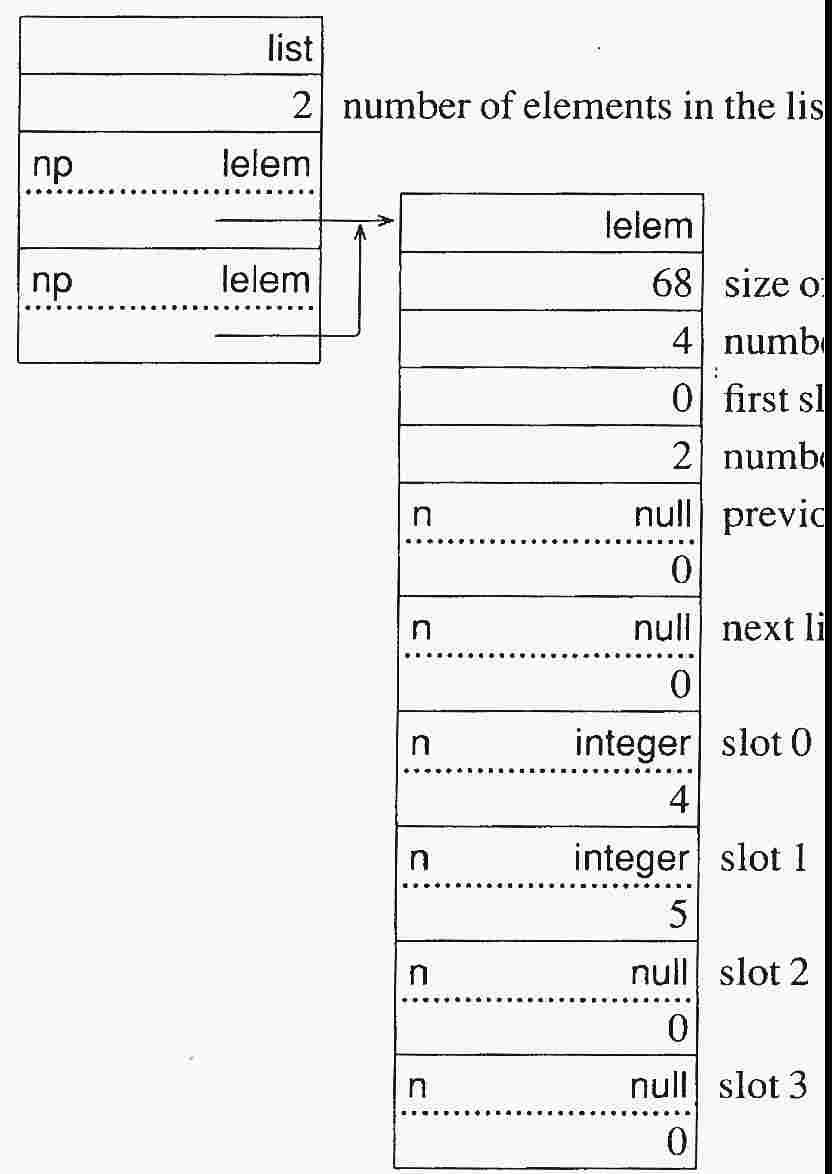
\includegraphics[width=2.778in,height=3.8417in]{ib-img/ib-img028.jpg} 
\begin{picture}(300,310)(0,32)
\begin{picture}(0,0)(0,-32)
\put(130,0){\dvbox{null}{n}{0}}
\put(130,0){\trboxlabel{slot 3}}
\put(130,32){\dvbox{null}{n}{0}}
\put(130,32){\trboxlabel{slot 2}}
\put(130,64){\dvbox{integer}{n}{5}}
\put(130,64){\trboxlabel{slot 1}}
\put(130,96){\dvbox{integer}{n}{4}}
\put(130,96){\trboxlabel{slot 0}}
\end{picture}
\put(130,160){\nullptrbox{next list-element block}}
\put(130,176){\nullptrbox{previous list-element block}}
\put(130,192){\blkbox{0}{2}}
\put(130,192){\rightboxlabels{first slot used}{number of slots used}}
\put(130,224){\blkbox{60}{4}}
\put(130,224){\rightboxlabels{size of block}{number of slots in block}}
\put(130,256){\wordbox{lelem}{}}
%
\put(0,240){\leftboxlabels{head}{tail}}
\put(0,240){\wordbox{}}
\put(0,240){\ruptr{36}{16}}
\put(0,256){\wordptr{50}{}}
\put(0,272){\wordbox{\textit{id}}}
\put(0,288){\blkbox{list}{2}}
\put(0,288){\brboxlabel{number of elements in the list}}
{\color{blue}
\put(366,168){\line(1,0){60}}
\put(426,168){\line(0,1){160}}
\put(426,328){\vector(-1,0){130}}
\put(296,328){\line(-1,0){316}}
\put(-20,328){\line(0,-1){16}}
\put(-20,312){\vector(1,0){20}}
\multiput(130,168)(4,0){23}{\line(1,0){2}}
\put(130,160){\blboxlabel{(Unicon) pointer to list header}}
}
\end{picture}

\ \ \ \ The List Element-Block after a put

Note that the increase in the number of elements in the header block
and in the number of slots used in the list-element block.

If an element is added to the beginning of a list, as in

%-% {\ttfamily\mdseries
%-% \ \ \ push(a,3)}
\iconline{
\>push(a,3)
}

\noindent the elements of the list are 3, 4, and 5. The new element is
put at the '{\textquotedbl}beginning{\textquotedbl} of the first
list-element block. The result is

%--%\ \  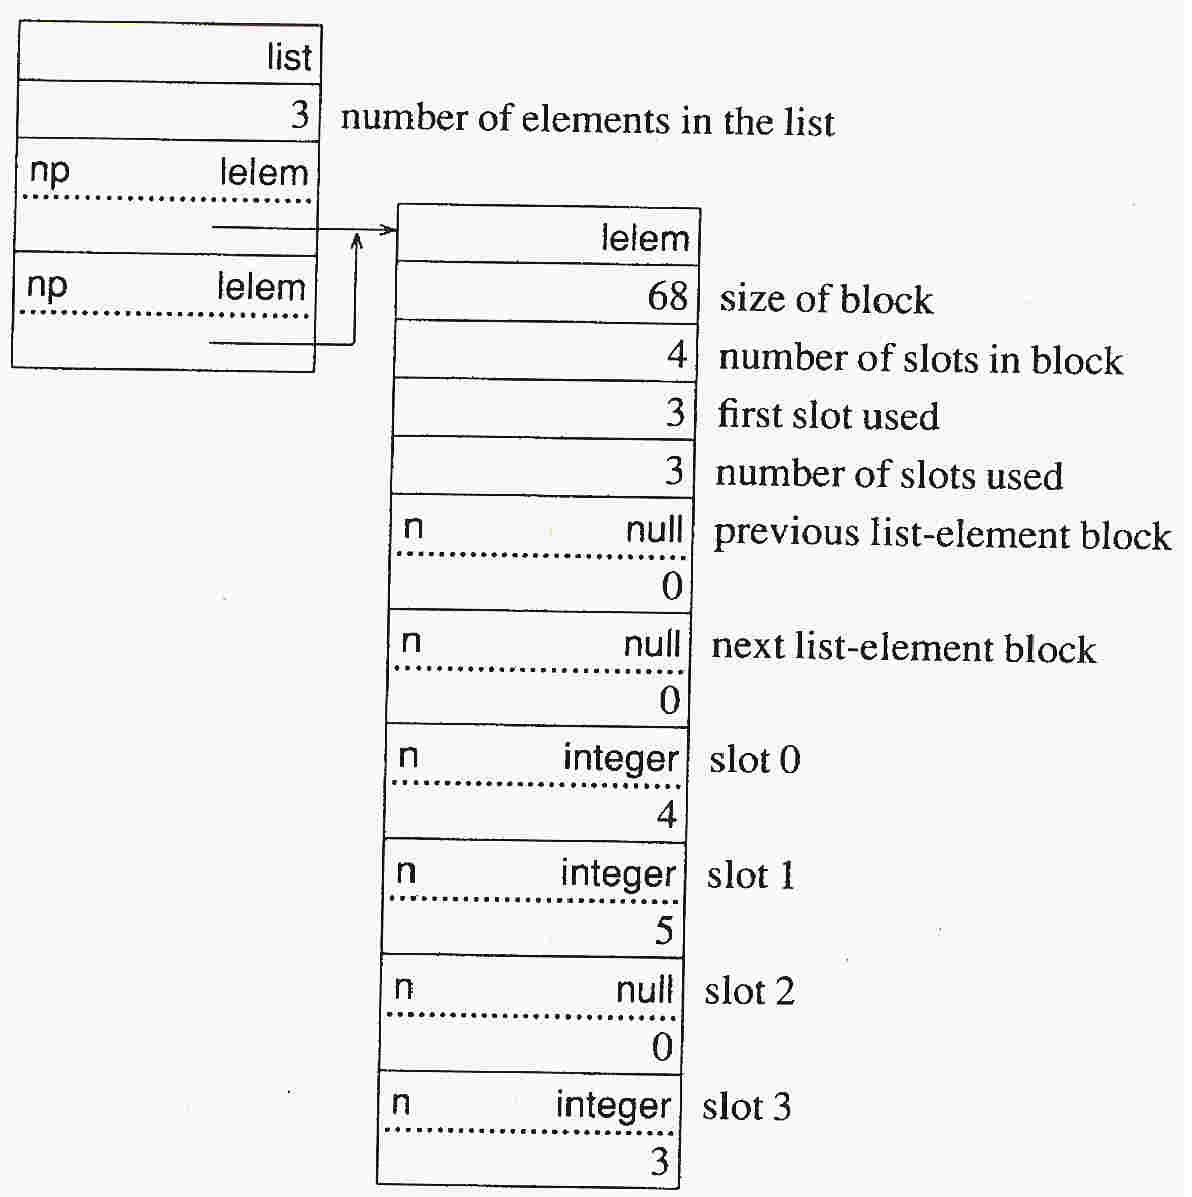
\includegraphics[width=4.0602in,height=3.8791in]{ib-img/ib-img029.jpg} 
\begin{picture}(300,310)(0,32)
\begin{picture}(0,0)(0,-32)
\put(130,0){\dvbox{integer}{n}{3}}
\put(130,0){\trboxlabel{slot 3}}
\put(130,32){\dvbox{null}{n}{0}}
\put(130,32){\trboxlabel{slot 2}}
\put(130,64){\dvbox{integer}{n}{5}}
\put(130,64){\trboxlabel{slot 1}}
\put(130,96){\dvbox{integer}{n}{4}}
\put(130,96){\trboxlabel{slot 0}}
\end{picture}
\put(130,160){\nullptrbox{next list-element block}}
\put(130,176){\nullptrbox{previous list-element block}}
\put(130,192){\blkbox{3}{3}}
\put(130,192){\rightboxlabels{first slot used}{number of slots used}}
\put(130,224){\blkbox{60}{4}}
\put(130,224){\rightboxlabels{size of block}{number of slots in block}}
\put(130,256){\wordbox{lelem}{}}
%
\put(0,240){\leftboxlabels{head}{tail}}
\put(0,240){\wordbox{}}
\put(0,240){\ruptr{36}{16}}
\put(0,256){\wordptr{50}{}}
\put(0,272){\wordbox{\textit{id}}}
\put(0,288){\blkbox{list}{3}}
\put(0,288){\brboxlabel{number of elements in the list}}
{\color{blue}
\put(366,168){\line(1,0){60}}
\put(426,168){\line(0,1){160}}
\put(426,328){\vector(-1,0){130}}
\put(296,328){\line(-1,0){316}}
\put(-20,328){\line(0,-1){16}}
\put(-20,312){\vector(1,0){20}}
\multiput(126,168)(4,0){23}{\line(1,0){2}}
\put(126,160){\blboxlabel{(Unicon) pointer to list header}}
}
\end{picture}

\ \ \ \ The List Element-Block after a push

Note that the {\textquotedbl}beginning,{\textquotedbl} which is before
the first physical slot in the list-element block, is the last
physical slot. The locations of elements that are in a list-element
block are determined by the three integers at the head of the list
element block. {\textquotedbl}Removal{\textquotedbl} of an element by
a pop, get, or pull does not shorten the list-element block or
overwrite the element; the element merely becomes inaccessible.

If an element is added to a list and no more slots are available in the
appropriate list-element block, a new list-element block is allocated and
linked in. The size of the new block is half the number of elements in the
entire list before expansion or \texttt{MinListSlots}, whichever is
greater.
{\color{blue} Unicon also imposes an upper limit of \texttt{MaxListSlots}
on the size of the new block.}
However, if there is not enough memory to allocate a list-element
block of the desired size, the size is reduced to fit into available
memory. For example, following evaluation of

%-% {\ttfamily\mdseries
%-% \ \ \ push(a.2)}
\iconline{
\>push(a,2)
}

%-% {\ttfamily\mdseries
%-% \ \ \ push(a.1)}
\iconline{
\>push(a,1)
}

\noindent the list elements are 1,2,3,4, and 5. The resulting structures are


%--% 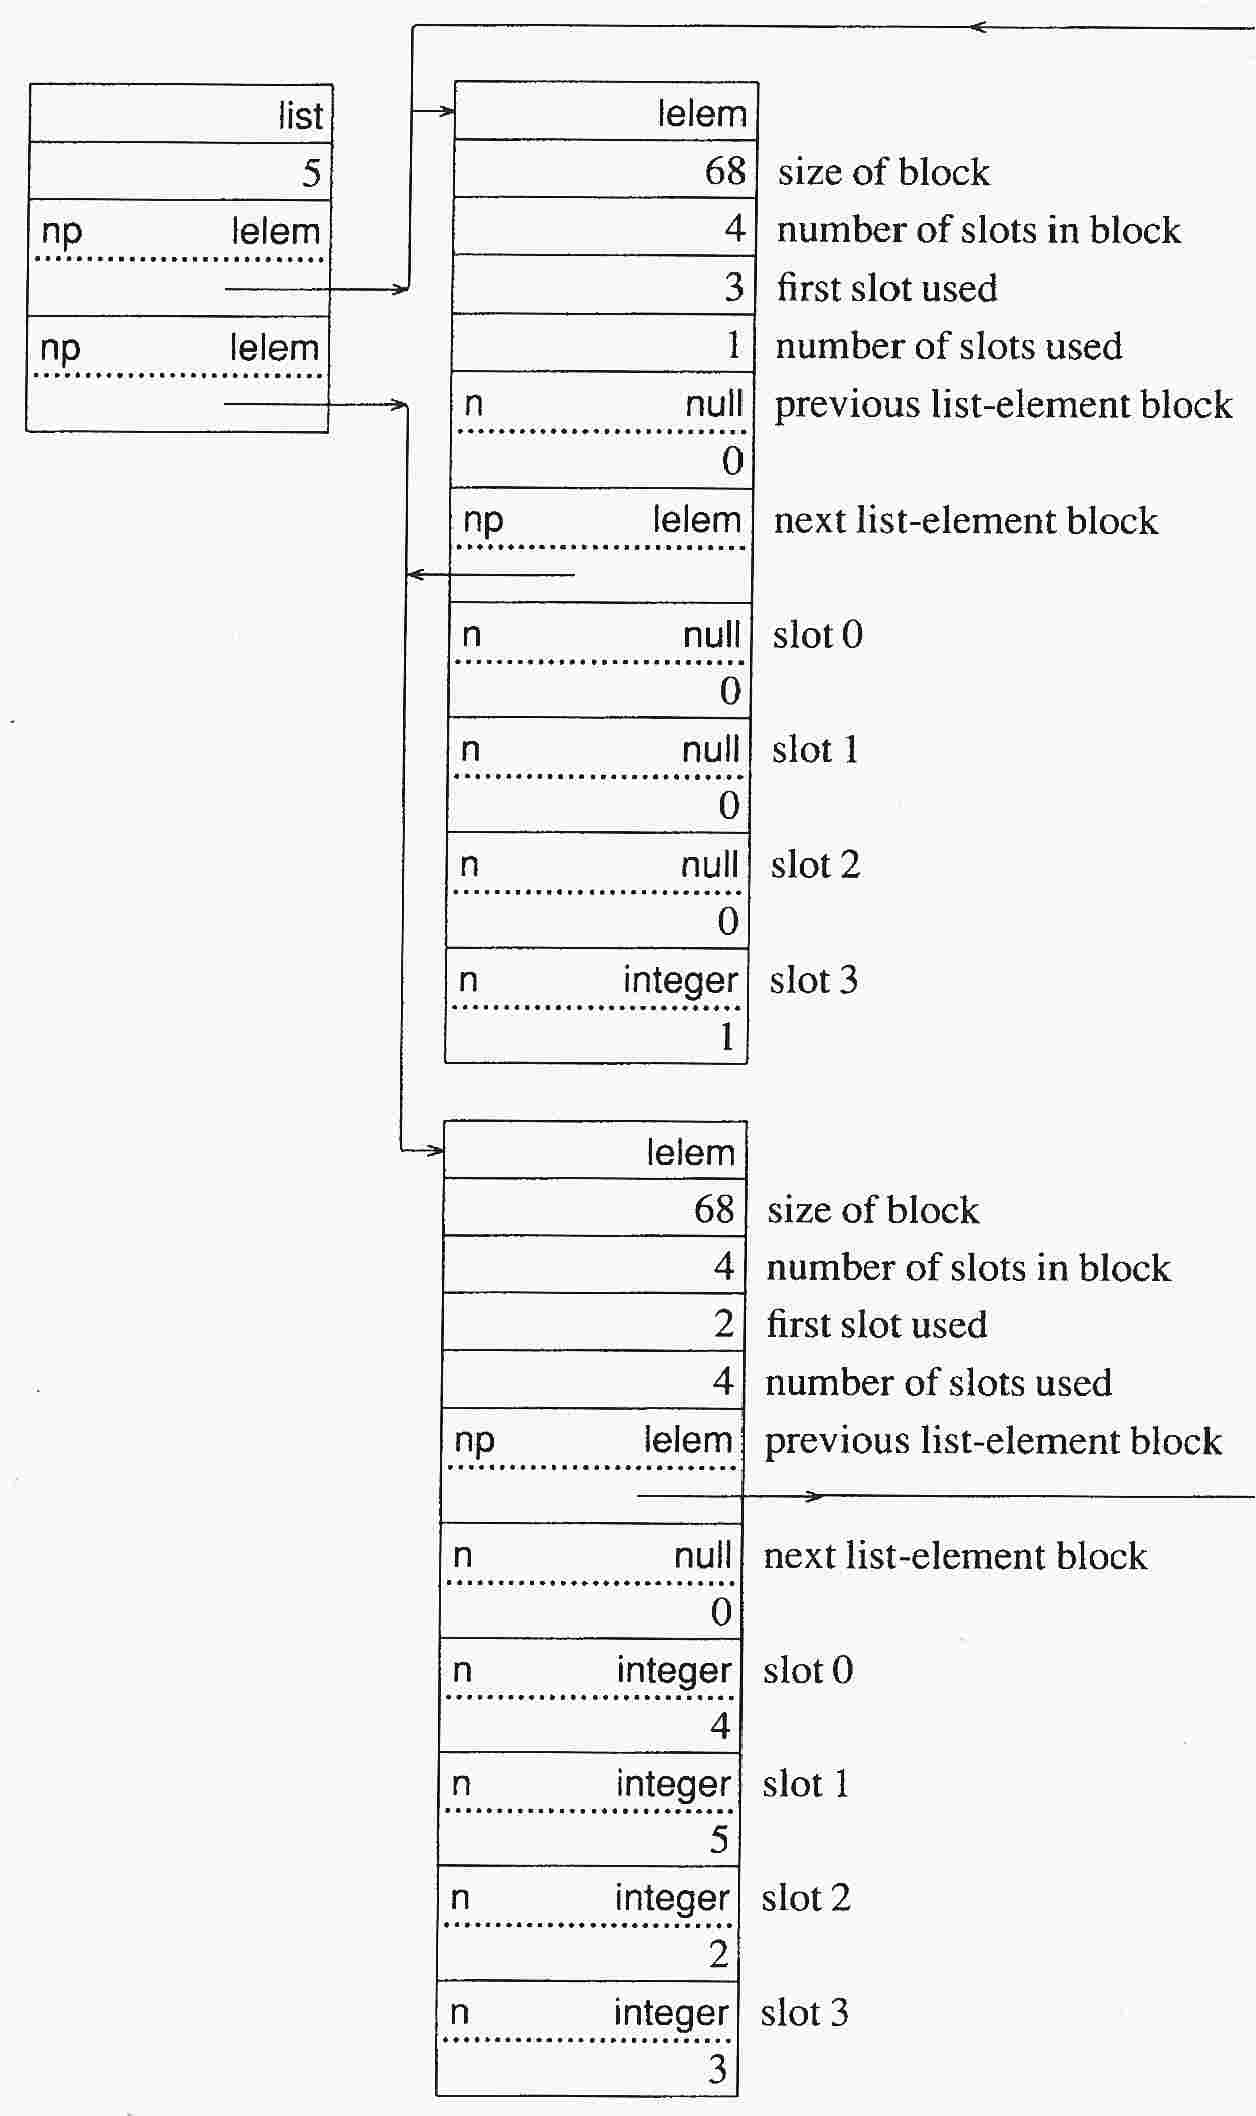
\includegraphics[width=4.2752in,height=6.9661in]{ib-img/ib-img030.jpg} \newline
\begin{picture}(300,520)
%
\put(0,256){% The top list block
\begin{picture}(300,300)
\put(130,0){\dvbox{integer}{n}{1}}
\put(130,0){\trboxlabel{slot 3}}
\put(130,32){\dvbox{null}{n}{0}}
\put(130,32){\trboxlabel{slot 2}}
\put(130,64){\dvbox{null}{n}{0}}
\put(130,64){\trboxlabel{slot 1}}
\put(130,96){\dvbox{null}{n}{0}}
\put(130,96){\trboxlabel{slot 0}}
\put(130,128){\wordbox{}}
\put(130,128){\brboxlabel{next list-element block}}
\put(130,128){\lptr{38}}
\put(130,144){\nullptrbox{previous list-element block}}
\put(130,160){\blkbox{3}{1}}
\put(130,160){\rightboxlabels{first slot used}{number of slots used}}
\put(130,192){\blkbox{60}{4}}
\put(130,192){\rightboxlabels{size of block}{number of slots in block}}
\put(130,224){\wordbox{lelem}{}}
%
\put(0,160){\leftboxlabels{head}{tail}}
\put(0,160){\wordbox{}}
\put(0,176){\wordbox{}}
\put(0,176){\ruptr{32}{16}}
\put(112,200){\line(0,1){32}}
\put(112,232){\vector(1,0){18}}
\put(0,192){\wordbox{\textit{id}}}
\put(0,208){\blkbox{list}{5}}
\put(0,160){\rdptr{32}{100}}
\put(112,68){\line(0,-1){68}}
\put(414,0){\line(0,1){252}}
\put(414,252){\vector(-1,0){100}}
\put(314,252){\line(-1,0){202}}
\put(112,252){\line(0,-1){20}}
{\color{blue}
\put(-44,0){\line(0,1){232}}
\put(-44,232){\vector(1,0){44}}
}
\end{picture}
}
\put(0,0){% The bottom list block
\begin{picture}(300,370)
\put(130,0){\dvbox{integer}{n}{3}}
\put(130,0){\trboxlabel{slot 3}}
\put(130,32){\dvbox{integer}{n}{2}}
\put(130,32){\trboxlabel{slot 2}}
\put(130,64){\dvbox{integer}{n}{5}}
\put(130,64){\trboxlabel{slot 1}}
\put(130,96){\dvbox{integer}{n}{4}}
\put(130,96){\trboxlabel{slot 0}}
\put(130,128){\nullptrbox{next list-element block}}
\put(310,144){\ruptr{24}{104}}
\put(130,144){\wordptr{30}{previous list-element block}}
\put(130,160){\blkbox{2}{4}}
\put(130,160){\rightboxlabels{first slot used}{number of slots used}}
\put(130,192){\blkbox{60}{4}}
\put(130,192){\rightboxlabels{size of block}{number of slots in block}}
\put(130,224){\wordbox{lelem}{}}
\put(112,232){\line(0,1){24}}
\put(112,232){\vector(1,0){18}}
{\color{blue}
\put(140,128){\luptr{204}{120}}
\put(120,144){\makebox(0,0)[r]{(Unicon) pointer to list header}}
}
\end{picture}
}
\end{picture}


\ \ The Addition of a List-Element Block


As elements are removed from a list by pop (which is synonymous with
get) or pull. The indices in the appropriate list-element block are
adjusted. The code for pop is

%-% {\ttfamily\mdseries
%-% int c\_get(hp, res)}
%-% 
%-% {\ttfamily\mdseries
%-% struct b\_list *hp;}
%-% 
%-% {\ttfamily\mdseries
%-% struct descrip *res;}
%-% 
%-% {\ttfamily\mdseries
%-% \{}
%-% 
%-% {\ttfamily\mdseries
%-% \ \ \ register word i;}
%-% 
%-% {\ttfamily\mdseries
%-% \ \ \ register struct b\_lelem *bp;}
%-% 
%-% 
%-% \bigskip
%-% 
%-% {\ttfamily\mdseries
%-% \ \ \ /*}
%-% 
%-% {\ttfamily\mdseries
%-% \ \ \ \ * Fail if the list is empty.}
%-% 
%-% {\ttfamily\mdseries
%-% \ \ \ \ */}
%-% 
%-% {\ttfamily\mdseries
%-% \ \ \ if (hp-{\textgreater}size {\textless}= 0)}
%-% 
%-% {\ttfamily\mdseries
%-% \ \ \ \ \ \ return 0;}
%-% 
%-% 
%-% \bigskip
%-% 
%-% {\ttfamily\mdseries
%-% \ \ \ /*}
%-% 
%-% {\ttfamily\mdseries
%-% \ \ \ \ * Point bp at the first list block. \ If the first block has}
%-% 
%-% {\ttfamily\mdseries
%-% \ \ \ \ * \ no elements in use, point bp at the next list block.}
%-% 
%-% {\ttfamily\mdseries
%-% \ \ \ \ */}
%-% 
%-% {\ttfamily\mdseries
%-% \ \ \ bp = (struct b\_lelem *) hp-{\textgreater}listhead;}
%-% 
%-% {\ttfamily\mdseries
%-% \ \ \ if (bp-{\textgreater}nused {\textless}= 0) \{}
%-% 
%-% {\ttfamily\mdseries
%-% \ \ \ \ \ \ bp = (struct b\_lelem *) bp-{\textgreater}listnext;}
%-% 
%-% {\ttfamily\mdseries
%-% \ \ \ \ \ \ hp-{\textgreater}listhead = (union block *) bp;}
%-% 
%-% {\ttfamily\mdseries
%-% \ \ \ \ \ \ bp-{\textgreater}listprev = NULL;}
%-% 
%-% {\ttfamily\mdseries
%-% \ \ \ \ \ \ \}}
%-% 
%-% 
%-% \bigskip
%-% 
%-% {\ttfamily\mdseries
%-% \ \ \ /*}
%-% 
%-% {\ttfamily\mdseries
%-% \ \ \ \ * Locate first element and assign it to result for return.}
%-% 
%-% {\ttfamily\mdseries
%-% \ \ \ \ */}
%-% 
%-% {\ttfamily\mdseries
%-% \ \ \ i = bp-{\textgreater}first;}
%-% 
%-% {\ttfamily\mdseries
%-% \ \ \ *res = bp-{\textgreater}lslots[i];}
%-% 
%-% 
%-% \bigskip
%-% 
%-% {\ttfamily\mdseries
%-% \ \ \ /*}
%-% 
%-% {\ttfamily\mdseries
%-% \ \ \ \ * Set bp-{\textgreater}first to new first element, or 0 if the block is}
%-% 
%-% {\ttfamily\mdseries
%-% \ \ \ \ * \ now empty. \ Decrement the usage count for the block and}
%-% 
%-% {\ttfamily\mdseries
%-% \ \ \ \ * \ the size of the list.}
%-% 
%-% {\ttfamily\mdseries
%-% \ \ \ \ */}
%-% 
%-% {\ttfamily\mdseries
%-% \ \ \ if (++i {\textgreater}= bp-{\textgreater}nslots)}
%-% 
%-% {\ttfamily\mdseries
%-% \ \ \ \ \ \ i = 0;}
%-% 
%-% {\ttfamily\mdseries
%-% \ \ \ bp-{\textgreater}first = i;}
%-% 
%-% {\ttfamily\mdseries
%-% \ \ \ bp-{\textgreater}nused-{}-;}
%-% 
%-% {\ttfamily\mdseries
%-% \ \ \ hp-{\textgreater}size-{}-;}
%-% 
%-% {\ttfamily\mdseries
%-% \ \ \ return 1;}
%-% 
%-% {\ttfamily\mdseries
%-% \}}
\iconcode{
int c\_get(hp, res)\\
struct b\_list *hp;\\
struct descrip *res;\\
\{\\
\>register word i;\\
\>register struct b\_lelem *bp;\\
\\
\>/*\\
\>\ * Fail if the list is empty.\\
\>\ */\\
\>if (hp->size <= 0)\\
\>\>return 0;\\
\\
\>/*\\
\>\ * Point bp at the first list block. \ If the first block has\\
\>\ * \ no elements in use, point bp at the next list block.\\
\>\ */\\
\>bp = (struct b\_lelem *) hp->listhead;\\
\>if (bp->nused <= 0) \{\\
\>\>bp = (struct b\_lelem *) bp->listnext;\\
\>\>hp->listhead = (union block *) bp;\\
\>\>bp->listprev = NULL;\\
\>\>\}\\
\\
\>/*\\
\>\ * Locate first element and assign it to result for return.\\
\>\ */\\
\>i = bp->first;\\
\>*res = bp->lslots[i];\\
\\
\>/*\\
\>\ * Set bp->first to new first element, or 0 if the block is\\
\>\ * \ now empty. \ Decrement the usage count for the block and\\
\>\ * \ the size of the list.\\
\>\ */\\
\>if (++i >= bp->nslots)\\
\>\>i = 0;\\
\>bp->first = i;\\
\>bp->nused-{}-;\\
\>hp->size-{}-;\\
\>return 1;\\
\}
}

\noindent where the \texttt{c\_get()} helper function is invoked from RTL as follows:

%-% {\ttfamily\mdseries
%-% function\{0,1\} get\_or\_pop(x)}
%-% 
%-% {\ttfamily\mdseries
%-% \ \ \ if !is:list(x) then}
%-% 
%-% {\ttfamily\mdseries
%-% \ \ \ \ \ \ runerr(108, x)}
%-% 
%-% 
%-% \bigskip
%-% 
%-% {\ttfamily\mdseries
%-% \ \ \ abstract \{}
%-% 
%-% {\ttfamily\mdseries
%-% \ \ \ \ \ \ return store[type(x).lst\_elem]}
%-% 
%-% {\ttfamily\mdseries
%-% \ \ \ \ \ \ \}}
%-% 
%-% 
%-% \bigskip
%-% 
%-% {\ttfamily\mdseries
%-% \ \ \ body \{}
%-% 
%-% {\ttfamily\mdseries
%-% \ \ \ \ \ \ if (!c\_get((struct b\_list *)BlkLoc(x), \&result)) fail;}
%-% 
%-% {\ttfamily\mdseries
%-% \ \ \ \ \ \ return result;}
%-% 
%-% {\ttfamily\mdseries
%-% \ \ \ \ \ \ \}}
%-% 
%-% {\ttfamily\mdseries
%-% end}
\iconcode{
function\{0,1\} get\_or\_pop(x)\\
\>if !is:list(x) then\\
\>\>runerr(108, x)\\
\\
\>abstract \{\\
\>\>return store[type(x).lst\_elem]\\
\>\>\}\\
\\
\>body \{\\
\>\>if (!c\_get((struct b\_list *)BlkLoc(x), \&result)) fail;\\
\>\>return result;\\
\>\>\}\\
end
}

Thus, as a result of

%-% {\ttfamily\mdseries
%-% \ \ \ pop(a)}
\iconline{
\>pop(a)
}

\noindent
the list elements are 2, 3, 4, and 5. The resulting structures are


%--%\ \  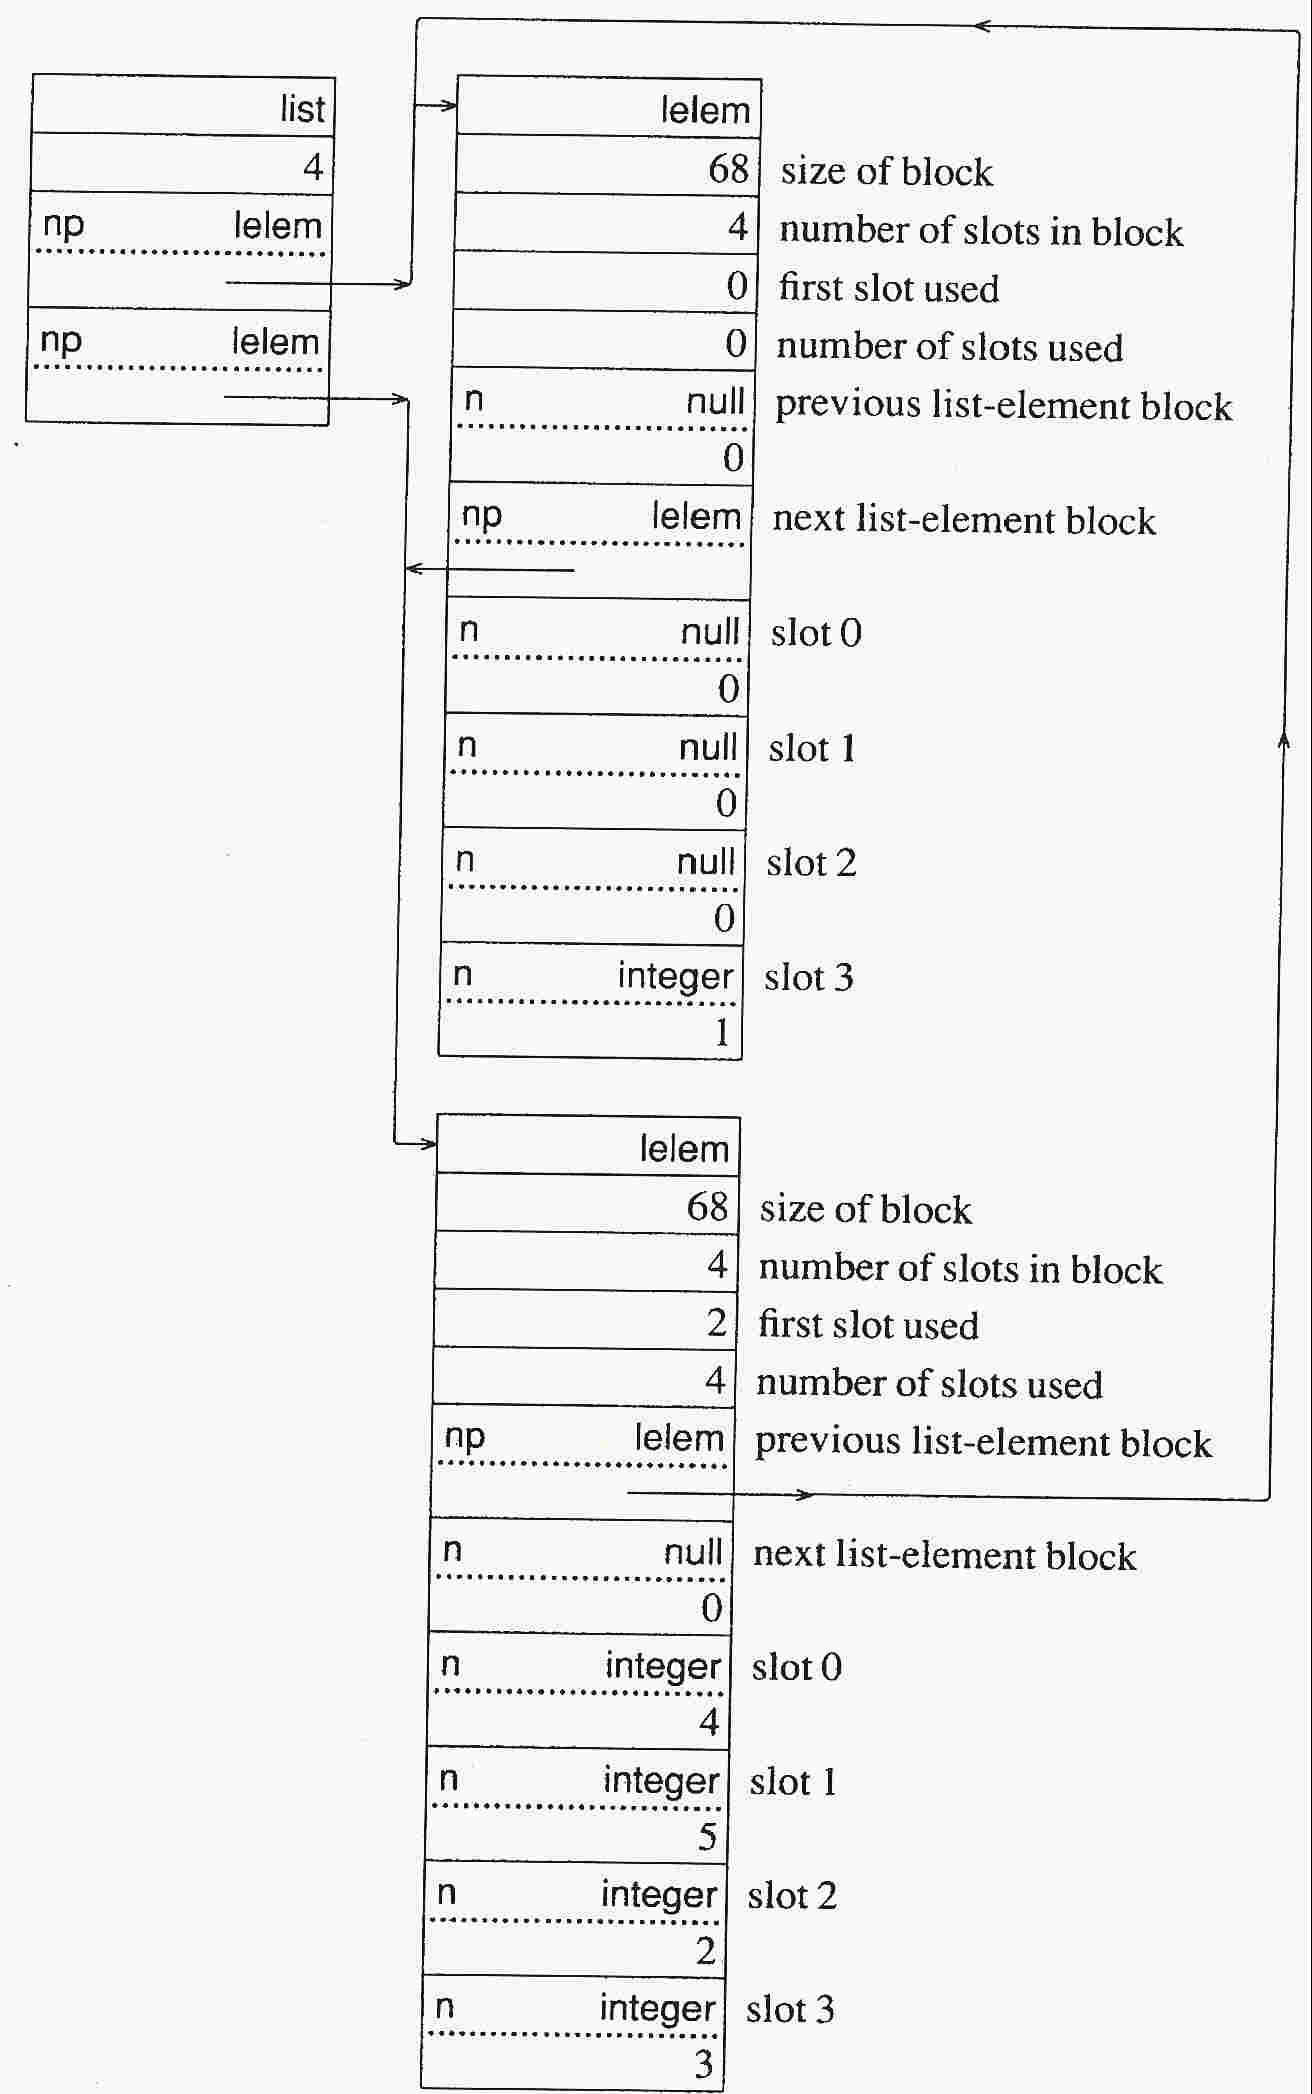
\includegraphics[width=4.3811in,height=6.9937in]{ib-img/ib-img031.jpg} 
\begin{picture}(300,520)
%
\put(0,256){% The top list block
\begin{picture}(300,300)
\put(130,0){\dvbox{integer}{n}{1}}
\put(130,0){\trboxlabel{slot 3}}
\put(130,32){\dvbox{null}{n}{0}}
\put(130,32){\trboxlabel{slot 2}}
\put(130,64){\dvbox{null}{n}{0}}
\put(130,64){\trboxlabel{slot 1}}
\put(130,96){\dvbox{null}{n}{0}}
\put(130,96){\trboxlabel{slot 0}}
\put(130,128){\wordbox{}}
\put(130,128){\brboxlabel{next list-element block}}
\put(130,128){\lptr{38}}
\put(130,144){\nullptrbox{previous list-element block}}
\put(130,160){\blkbox{0}{0}}
\put(130,160){\rightboxlabels{first slot used}{number of slots used}}
\put(130,192){\blkbox{60}{4}}
\put(130,192){\rightboxlabels{size of block}{number of slots in block}}
\put(130,224){\wordbox{lelem}{}}
%
\put(0,160){\leftboxlabels{head}{tail}}
\put(0,160){\wordbox{}}
\put(0,176){\wordbox{}}
\put(0,176){\ruptr{32}{16}}
\put(112,200){\line(0,1){32}}
\put(112,232){\vector(1,0){18}}
\put(0,192){\wordbox{\textit{id}}}
\put(0,208){\blkbox{list}{4}}
\put(0,160){\rdptr{32}{100}}
\put(112,68){\line(0,-1){68}}
\put(414,0){\line(0,1){252}}
\put(414,252){\vector(-1,0){100}}
\put(314,252){\line(-1,0){202}}
\put(112,252){\line(0,-1){20}}
{\color{blue}
\put(-44,0){\line(0,1){232}}
\put(-44,232){\vector(1,0){44}}
}
\end{picture}
}
\put(0,0){% The bottom list block
\begin{picture}(300,370)
\put(130,0){\dvbox{integer}{n}{3}}
\put(130,0){\trboxlabel{slot 3}}
\put(130,32){\dvbox{integer}{n}{2}}
\put(130,32){\trboxlabel{slot 2}}
\put(130,64){\dvbox{integer}{n}{5}}
\put(130,64){\trboxlabel{slot 1}}
\put(130,96){\dvbox{integer}{n}{4}}
\put(130,96){\trboxlabel{slot 0}}
\put(130,128){\nullptrbox{next list-element block}}
\put(310,144){\ruptr{24}{104}}
\put(130,144){\wordptr{30}{previous list-element block}}
\put(130,160){\blkbox{2}{4}}
\put(130,160){\rightboxlabels{first slot used}{number of slots used}}
\put(130,192){\blkbox{60}{4}}
\put(130,192){\rightboxlabels{size of block}{number of slots in block}}
\put(130,224){\wordbox{lelem}{}}
\put(112,232){\line(0,1){24}}
\put(112,232){\vector(1,0){18}}
{\color{blue}
\put(140,128){\luptr{204}{120}}
\put(120,144){\makebox(0,0)[r]{(Unicon) pointer to list header}}
}
\end{picture}
}
\end{picture}

\ \ \ \ The Result of Removing Elements from a List-Element Block


Note that the first list-element block is still linked in the chain,
even though it no longer contains any elements that are logically
accessible. A list-element block is not removed from the chain when it
becomes empty. It is removed only when an element is removed from a
list that already has an empty list-element block. Thus, there is
always at least one list-element block on the chain, even if the list
is empty. Aside from simplifying the access to list-element blocks
from the list-header block, this strategy avoids repeated allocation
in the case that pop/push pairs occur at the boundary of two
list-element blocks.

Continuing the previous example,

%-% {\ttfamily\mdseries
%-% \ \ \ pop(a)}
\iconline{
\>pop(a)
}

\noindent leaves the list elements 3, 4, and 5. The empty list-element
block is removed from the chain:

%--% 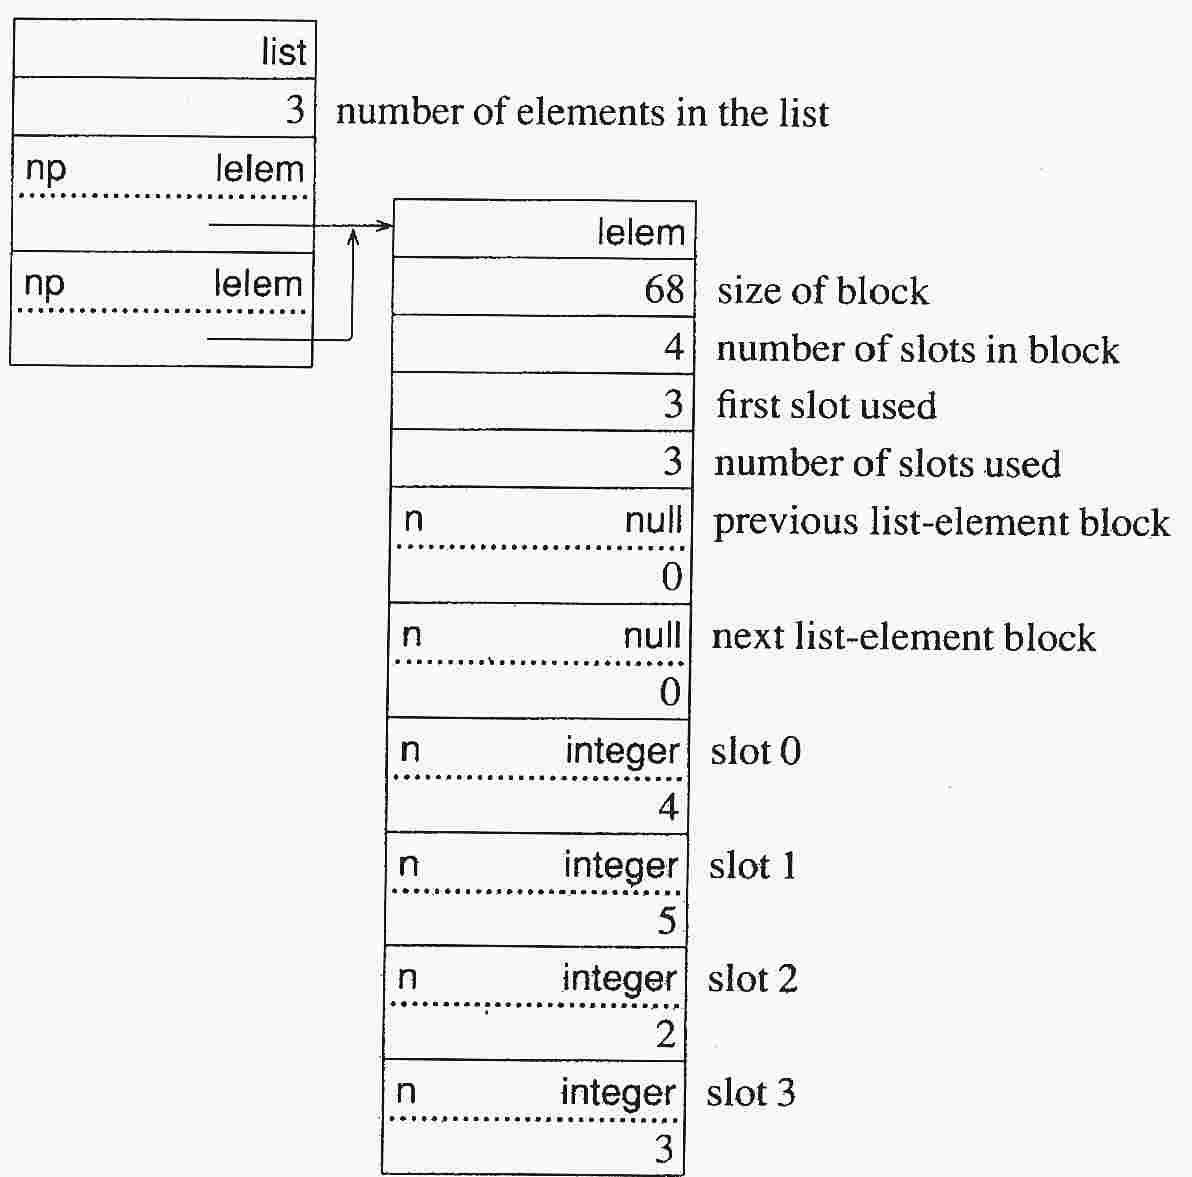
\includegraphics[width=4.0602in,height=3.9307in]{ib-img/ib-img032.jpg} 
\begin{picture}(300,310)(-20,0)
\put(130,0){\dvbox{integer}{n}{3}}
\put(130,0){\trboxlabel{slot 3}}
\put(130,32){\dvbox{integer}{n}{2}}
\put(130,32){\trboxlabel{slot 2}}
\put(130,64){\dvbox{integer}{n}{5}}
\put(130,64){\trboxlabel{slot 1}}
\put(130,96){\dvbox{integer}{n}{4}}
\put(130,96){\trboxlabel{slot 0}}
\put(130,128){\nullptrbox{next list-element block}}
\put(130,144){\nullptrbox{previous list-element block}}
%% \put(130,128){\dvbox{null}{n}{0}}
%% \put(130,128){\trboxlabel{next list-element block}}
%% \put(130,160){\dvbox{null}{n}{0}}
%% \put(130,160){\trboxlabel{previous list-element block}}

\put(130,160){\blkbox{3}{3}}
\put(130,160){\rightboxlabels{first slot used}{number of slots used}}
\put(130,192){\blkbox{60}{4}}
\put(130,192){\rightboxlabels{size of block}{number of slots in block}}
\put(130,224){\wordbox{lelem}{}}
%
\put(0,208){\leftboxlabels{head}{tail}}
\put(0,208){\wordbox{}}
\put(0,208){\ruptr{36}{16}}
\put(0,224){\wordptr{50}}
\put(0,240){\wordbox{\textit{id}}}
\put(0,256){\blkbox{list}{3}}
\put(0,256){\brboxlabel{number of elements in the list}}
{\color{blue}
\put(138,128){\luptr{200}{40}}
\put(-42,176){\line(0,1){104}}
\put(-42,280){\vector(1,0){42}}
\put(120,144){\makebox(0,0)[r]{(Unicon) pointer to list header}}
}
\end{picture}

\ \ Removal of an Empty List-Element Block

Note that the value 2 is still physically in the list-element block,
although it is logically inaccessible.

\section[6.3 Positional Access]{6.3 Positional Access}

Positional reference of the form \texttt{a[i]} requires locating the
correct list-element block. Out-of-range references can be determined
by examining the list-header block. If the list has several
list-element blocks, this involves linking through the list-element
blocks, while keeping track of the count of elements in each block
until the appropriate one is reached. The result of evaluating
\texttt{a[i]} is a variable that points to the appropriate slot.

The portion of the subscripting code that handles lists is

%-% {\ttfamily\mdseries
%-% \ \ \ type\_case dx of \{}
%-% 
%-% {\ttfamily\mdseries
%-% \ \ \ \ \ \ list: \{}
%-% 
%-% {\ttfamily\mdseries
%-% \ \ \ \ \ \ \ \ \ abstract \{}
%-% 
%-% {\ttfamily\mdseries
%-% \ \ \ \ \ \ \ \ \ \ \ \ return type(dx).lst\_elem}
%-% 
%-% {\ttfamily\mdseries
%-% \ \ \ \ \ \ \ \ \ \ \ \ \}}
%-% 
%-% {\ttfamily\mdseries
%-% \ \ \ \ \ \ \ \ \ /*}
%-% 
%-% {\ttfamily\mdseries
%-% \ \ \ \ \ \ \ \ \ \ * Make sure that y is a C integer.}
%-% 
%-% {\ttfamily\mdseries
%-% \ \ \ \ \ \ \ \ \ \ */}
%-% 
%-% {\ttfamily\mdseries
%-% \ \ \ \ \ \ \ \ \ if !cnv:C\_integer(y) then \{}
%-% 
%-% {\ttfamily\mdseries
%-% \ \  \ \ \ /*}
%-% 
%-% {\ttfamily\mdseries
%-% \ \  \ \ \ \ * If it isn't a C integer, but is a large integer,}
%-% 
%-% {\ttfamily\mdseries
%-% \ \  \ \ \ \ * fail on the out-of-range index.}
%-% 
%-% {\ttfamily\mdseries
%-% \ \  \ \ \ \ */}
%-% 
%-% {\ttfamily\mdseries
%-% \ \  \ \ \ if cnv : integer(y) then inline \{ fail; \}}
%-% 
%-% {\ttfamily\mdseries
%-% \ \  \ \ \ runerr(101, y)}
%-% 
%-% {\ttfamily\mdseries
%-% \ \  \ \ \ \}}
%-% 
%-% {\ttfamily\mdseries
%-% \ \ \ \ \ \ \ \ \ body \{}
%-% 
%-% {\ttfamily\mdseries
%-% \ \ \ \ \ \ \ \ \ \ \ \ word i, j;}
%-% 
%-% {\ttfamily\mdseries
%-% \ \ \ \ \ \ \ \ \ \ \ \ register union block *bp; /* no need to be tended */}
%-% 
%-% {\ttfamily\mdseries
%-% \ \ \ \ \ \ \ \ \ \ \ \ struct b\_list *lp; \ \ \ /* doesn't need to be tended */}
%-% 
%-% 
%-% \bigskip
%-% 
%-% {\ttfamily\mdseries
%-% \ \  \ \ \ /*}
%-% 
%-% {\ttfamily\mdseries
%-% \ \  \ \ \ \ * Make sure that subscript y is in range.}
%-% 
%-% {\ttfamily\mdseries
%-% \ \  \ \ \ \ */}
%-% 
%-% {\ttfamily\mdseries
%-% \ \ \ \ \ \ \ \ \ \ \ \ lp = (struct b\_list *)BlkLoc(dx);}
%-% 
%-% {\ttfamily\mdseries
%-% \ \ \ \ \ \ \ \ \ \ \ \ i = cvpos((long)y, (long)lp-{\textgreater}size);}
%-% 
%-% {\ttfamily\mdseries
%-% \ \ \ \ \ \ \ \ \ \ \ \ if (i == CvtFail {\textbar}{\textbar} i {\textgreater} lp-{\textgreater}size)}
%-% 
%-% {\ttfamily\mdseries
%-% \ \ \ \ \ \ \ \ \ \ \ \ \ \ \ fail;}
%-% 
%-% {\ttfamily\mdseries
%-% \ \ \ \ \ \ \ \ \ \ \ \ /*}
%-% 
%-% {\ttfamily\mdseries
%-% \ \ \ \ \ \ \ \ \ \ \ \ \ * Locate the list-element block containing the}
%-% 
%-% {\ttfamily\mdseries
%-% \ \ \ \ \ \ \ \ \ \ \ \ \ * \ desired element.}
%-% 
%-% {\ttfamily\mdseries
%-% \ \ \ \ \ \ \ \ \ \ \ \ \ */}
%-% 
%-% {\ttfamily\mdseries
%-% \ \ \ \ \ \ \ \ \ \ \ \ bp = lp-{\textgreater}listhead;}
%-% 
%-% {\ttfamily\mdseries
%-% \ \ \ \ \ \ \ \ \ \ \ \ j = 1;}
%-% 
%-% {\ttfamily\mdseries
%-% \ \  \ \ \ /*}
%-% 
%-% {\ttfamily\mdseries
%-% \ \  \ \ \ \ * y is in range, so bp can never be null here. If it}
%-% 
%-% {\ttfamily\mdseries
%-% \ \  \ \ \ \ * was, a memory violation would occur in the code that}
%-% 
%-% {\ttfamily\mdseries
%-% \ \  \ \ \ \ * follows, anyhow, so exiting the loop on a NULL bp}
%-% 
%-% {\ttfamily\mdseries
%-% \ \  \ \ \ \ * makes no sense.}
%-% 
%-% {\ttfamily\mdseries
%-% \ \  \ \ \ \ */}
%-% 
%-% {\ttfamily\mdseries
%-% \ \  \ \ while (i {\textgreater}= j + bp-{\textgreater}lelem.nused) \{}
%-% 
%-% {\ttfamily\mdseries
%-% \ \  \ \ \ \ \ j += bp-{\textgreater}lelem.nused;}
%-% 
%-% {\ttfamily\mdseries
%-% \ \  \ \ \ \ \ bp = BlkLoc(bp-{\textgreater}lelem.listnext);}
%-% 
%-% {\ttfamily\mdseries
%-% \ \  \ \ \ \ \ \}}
%-% 
%-% 
%-% \bigskip
%-% 
%-% 
%-% \ \  \ \ /*
%-% 
%-% {\ttfamily
%-% \textrm{\ \  \ \ \ }* Locate desired element and return a pointer to it.}
%-% 
%-% {\ttfamily
%-% \ \  \ \ \ */}
%-% 
%-% {\ttfamily
%-% \ \  \ \ i += bp-{\textgreater}lelem.first - j;}
%-% 
%-% {\ttfamily
%-% \ \  \ \ if (i {\textgreater}= bp-{\textgreater}lelem.nslots)}
%-% 
%-% {\ttfamily
%-% \ \  \ \ \ \ \ i -= bp-{\textgreater}lelem.nslots;}
%-% 
%-% {\ttfamily
%-% \ \  \ \ return struct\_var(\&bp-{\textgreater}lelem.lslots[i], bp);}
%-% 
%-% {\ttfamily
%-% \ \  \ \ \}}
%-% 
%-% {\ttfamily
%-% \ \  \}}
\goodbreak
\iconcode{
\>type\_case dx of \{\\
\>\>list: \{\\
\>\>\>abstract \{\\
\>\>\>\>return type(dx).lst\_elem\\
\>\>\>\>\}\\
\>\>\>/*\\
\>\>\>\ * Make sure that y is a C integer.\\
\>\>\>\ */\\
\>\>\>if !cnv:C\_integer(y) then \{\\
\>\>/*\\
\>\>\ * If it isn't a C integer, but is a large integer,\\
\>\>\ * fail on the out-of-range index.\\
\>\>\ */\\
\>\>if cnv : integer(y) then inline \{ fail; \}\\
\>\>runerr(101, y)\\
\>\>\}\\
\>\>\>body \{\\
\>\>\>\>word i, j;\\
\>\>\>\>register union block *bp; /* no need to be tended */\\
\>\>\>\>struct b\_list *lp; \ \ \ /* doesn't need to be tended */\\
\\
\>\>/*\\
\>\>\ * Make sure that subscript y is in range.\\
\>\>\ */\\
\>\>\>\>lp = (struct b\_list *)BlkLoc(dx);\\
\>\>\>\>i = cvpos((long)y, (long)lp->size);\\
\>\>\>\>if (i == CvtFail || i > lp->size)\\
\>\>\>\>\>fail;\\
\>\>\>\>/*\\
\>\>\>\>\ * Locate the list-element block containing the\\
\>\>\>\>\ * \ desired element.\\
\>\>\>\>\ */\\
\>\>\>\>bp = lp->listhead;\\
\>\>\>\>j = 1;\\
\>\>/*\\
\>\>\ * y is in range, so bp can never be null here. If it\\
\>\>\ * was, a memory violation would occur in the code that\\
\>\>\ * follows, anyhow, so exiting the loop on a NULL bp\\
\>\>\ * makes no sense.\\
\>\>\ */\\
\>\ \ while (i >= j + bp->lelem.nused) \{\\
\>\>\ \ j += bp->lelem.nused;\\
\>\>\ \ bp = BlkLoc(bp->lelem.listnext);\\
\>\>\ \ \}\\
\\
\>\>/*\\
\>\>* Locate desired element and return a pointer to it.\\
\>\>*/\\
\>\>i += bp->lelem.first - j;\\
\>\>if (i >= bp->lelem.nslots)\\
\>\>\>i -= bp->lelem.nslots;\\
\>\>return struct\_var(\&bp->lelem.lslots[i], bp);\\
\>\>\}\\
\>\}
}

For the preceding example, \texttt{a[3]} produces a variable that
points indirectly to the descriptor for the value 5:

%--% 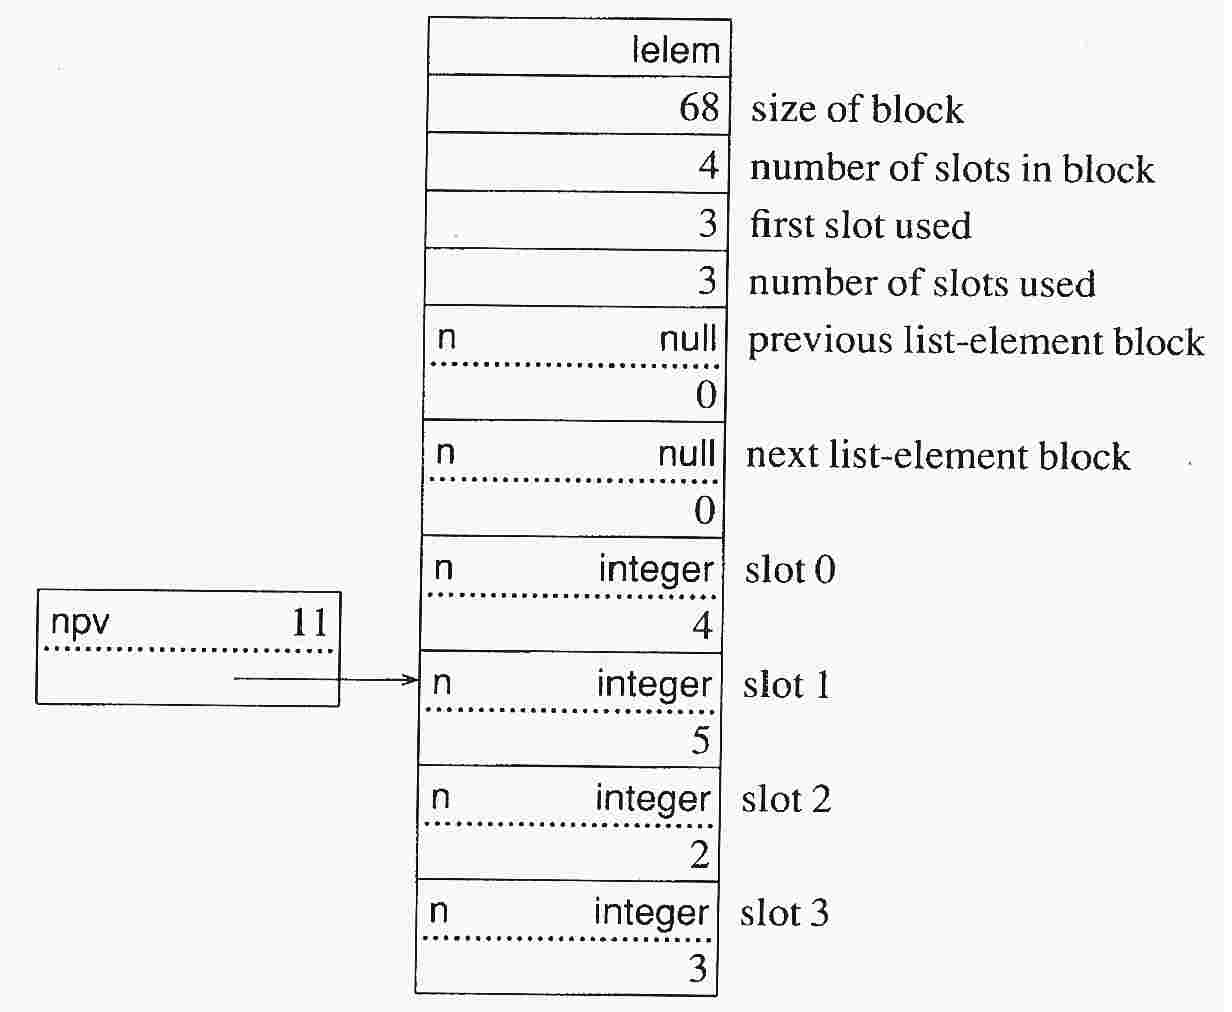
\includegraphics[width=4.1681in,height=3.3799in]{ib-img/ib-img033.jpg} 
\begin{picture}(300,250)(-20,0)
\put(140,0){\dvbox{integer}{n}{3}}
\put(140,0){\trboxlabel{slot 3}}
\put(140,32){\dvbox{integer}{n}{2}}
\put(140,32){\trboxlabel{slot 2}}
\put(140,64){\dvbox{integer}{n}{5}}
\put(140,64){\trboxlabel{slot 1}}
\put(140,96){\dvbox{integer}{n}{4}}
\put(140,96){\trboxlabel{slot 0}}
\put(140,128){\nullptrbox{next list-element block}}
\put(140,144){\nullptrbox{previous list-element block}}
\put(140,160){\blkbox{3}{3}}
\put(140,160){\rightboxlabels{first slot used}{number of slots used}}
\put(140,192){\blkbox{60}{4}}
\put(140,192){\rightboxlabels{size of block}{number of slots in block}}
\put(140,224){\wordbox{lelem}{}}
%
\put(0,80){\dvptrbox{9}{npv}{40}{}}
\put(120,88){\line(0,1){144}}
\put(120,232){\vector(1,0){20}}
\multiput(120,88)(4,0){4}{\line(1,0){2}}
\put(136,88){\vector(1,0){4}}
{\color{blue}
\multiput(126,136)(4,0){26}{\line(1,0){2}}
\put(126,128){\blboxlabel{(Unicon) pointer to list header}}
}
\end{picture}

\ \ \ \ Referencing a List Element

Note the offset of nine words in the d-word of the variable.  In version 6 of
Icon the descriptor pointed directly at the variable and the offset enabled the
garbage collector to locate the top of the block. In current versions of Icon
and Unicon the variable points to the top of the block and the offset enables
the correct list-element to be referenced. This change was necessitated by the
introduction of block pointers --- see Chapter 11 for details.

\section[6.4 Arrays (Unicon only)]{6.4 Arrays (Unicon only)}

The Unicon language provides a special case of the general list structure
that is optimized for fast access to the list-elements. An array is a list
where all the list-elements are the same numeric type and are in a single
block. It is created by calling

\iconline{array($dimen$, $value$)}

\noindent which will return a one dimensional ``vector'' of $dimen$
elements that are all set to $value$.  $value$ may be a small integer or
a floating point value. It may also be a list, in which case the value for
the array is the value of the first element of the list.

%% [DonW] To check (in the source):
%% What happens when a descriptor is needed (eg. a procedure returns an
%% integer value that may be assigned to)?
%%        A descriptor is built by calling struct_var
%% What happens when a real value is assigned to an integer array and vice-versa?
%%        The code for the assignment operator checks the type of the header block
%%        to see if it's an array. If so it converts the array to a list of the
%%        type changes.
%% What do array slices do?
%%
%% Does the garbage collector need to know about arrays? I suspect yes
%%        No special treatment is required for arrays
%% What happens if an assignment is made beyond the end of the array?
%%        It should fail, but strange things happen.

For example, following evaluation of

\iconline{vec := array(100,42)}

\noindent 
there will be 100 integers in the array, all set to 42.
The resulting structures are

\begin{picture}(400,260)(0,-10)
\begin{picture}(0,0)(-145,0)
\put(120,0){\blkbox{42}{42}}
\put(129,0){\blboxlabel{\texttt{vec[100]}}}
\put(129,0){\tlboxlabel{\texttt{vec[99]}}}
\put(120,0){\upetc}
\put(100,50){\vdots}
\put(120,80){\downetc}
\put(120,80){\blkbox{42}{42}}
\put(120,80){\tlboxlabel{\texttt{vec[1]}}}
\put(120,80){\blboxlabel{\texttt{vec[2]}}}
\put(120,112){\nullptrbox{dims}}
\put(120,128){\wordbox{}{}}
\put(115,184){\makebox(100,0)[l]{First (and only) list-element block}}
\put(120,144){\blkbox{intarray}{416}}
\put(120,144){\brboxlabel{size (bytes)}}
\end{picture}
\put(130,232){\makebox(108,0){List header block}}
\put(130,144){\nullptrbox{}}
\put(130,160){\blkptrbox{\textit{id}}{55}{}}
\put(130,192){\blkbox{list}{100}}
\put(-5,208){\dvptrbox{list}{npv}{54}{}}
\put(-5,208){\tlboxlabel{\texttt{vec}}}
\put(450,216){\vector(-1,0){219}}
\put(450,216){\line(0,-1){80}}
\put(450,136){\line(-1,0){100}}
\end{picture}

At present (January 2017) multi-dimensional arrays are not supported,
although there is provision in the data structures for more than one
dimension. Multi dimensional arrays will be created by calling

\iconline{array($dimen_1$, $dimen_2$, \dots , $dimen_n$, $value$)}

The only change to the diagram above will be that the null pointer in the
\texttt{dims} field will be replaced by a pointer to another intarray block
that contains each of the values $dimen_1$ \dots $dimen_n$.

Provided that the elements in the array are only assigned values of the
same initial type, they will stay together in one contiguous block and
enjoy the benefits of faster access. If a value of a different type is
assigned or an array element is deleted, or the array is extended (by
\texttt{push} or \texttt{put}) the runtime system converts the array into a
conventional list. The code extract to convert an integer array to a list
(taken from the \texttt{asgn} operator) is below.  In the extract,
\texttt{x} is a descriptor that points to the array element and \texttt{y}
is a descriptor that points to the new value.

\goodbreak
\iconcode{
if (BlkD(x,Intarray)->title==T\_Intarray)\{\\
\>C\_integer ii;\\
\>if (cnv:(exact)C\_integer(y, ii)) \\
\>\> *((word *)VarLoc(x) + Offset(x)) = ii;\\
\>else\{ /* y is not integer, try to convert the intarray to list*/\\
\>\>   tended struct b\_list *xlist= BlkD(x, Intarray)->listp;\\
\>\>   tended struct descrip dlist;\\
\>\>   word i;\\
\>\>   \\
\>\>   i = (Offset(x)*sizeof(word)-sizeof(struct b\_intarray)+\\
\>\>  sizeof(word)) / sizeof(word);\\
\>\>   \\
\>\>   dlist.vword.bptr = (union block *) xlist;\\
\>\>   dlist.dword = D\_List;		     \\
\>\>   if (arraytolist(\&dlist)!=Succeeded) fail;\\
\>\>   \\
\>\>   /* \\
\>\>   * assuming the new list has one lelem block only, \\
\>\>   * i should be in the first block. no need to loop \\
\>\>   * through several blocks\\
\>\>   */\\
\>\>\\
\>\>   *(dptr)(\&xlist->listhead->Lelem.lslots[i]) = y;\\
\>  \}\\
\}
}

The code to convert an array of real values is very similar to the code for
integer arrays.

\bigskip\bigskip
\textsc{Retrospective}: The structures used for implementing lists are
relatively complicated, but they provide a reasonable compromise, both
in the utilization of storage and access speed, that accommodates
different access mechanisms.

Using a chain of list-element blocks allows lists to grow in size
without limit. From the viewpoint of positional access, this amounts
to segmentation. This segmentation only occurs, however, when elements
are added to a list. The use of circular queues within list-element
blocks allows elements to be removed and added without wasting space.

Arrays provide a useful speed-up in cases where the list elements are
numeric and the list does not grow or shrink.

\bigskip

\noindent\textbf{EXERCISES}

\liststyleLvi
\begin{enumerate}
\item \begin{enumerate}
\item 
Diagram the structures that result from the evaluation of the
following expressions:\newline
 graph := [{\textquotedbl}a{\textquotedbl},,]\newline
 graph[2] := graph[3] := graph

\item How much space does an empty list occupy?

\item The portions of the structures for a list that are not occupied
by elements of the list constitute overhead. Calculate the percentage
of overhead in the following lists. Assume that the minimum number of
slots in a list-element block is eight.\newline
 a := []\newline
 a := [1, 2]\newline
 a := [1, 2, 3, 4, 5]\newline
 a := list(100)\newline
 a := []; every put(a, 1 to 100)\newline
How do these figures vary as a function of the minimum number of slots
in a list-element block?

\item What are the implications of not ``zeroing'' list elements when
they are logically removed by a pop, get, or pull?

\item When a list-element block is unlinked as the result of a pop,
get, or pull, are the elements in it really inaccessible to the
source program?

\item There is considerable overhead involved in the implementation of
\textit{lists }to support both positional access and stack and queue
access mechanisms. Suppose the language were changed so that stack and
queue access mechanisms applied only to lists that were initially
empty. What would the likely impact be on existing Icon programs? How
could the implementation take advantage of this change?

\item As elements are added to lists, more list-element blocks are
added and they tend to become ``fragmented.'' Is it feasible to
reorganize such lists, combining the elements in many list-element
blocks into one large block? If when and how could this be done?

\item A suggested alternative to maintaining a chain of list-element
blocks is to allocate a larger block when space is needed and copy
elements from the previous block into it. Criticize this proposal.

\item Suppose it were possible to insert elements in the middle of
lists, rather than only at the ends. How might this feature be
implemented?

\end{enumerate}
\end{enumerate}
